% \title{How to reduce bureaucratic corruption? Unpacking Brazilian anti-corruption audits}
% \date{\today\thanks{
%     We thank Noah Buckley, Mark Buntaine, Dan Honig, Matias Iaryczower, Jenn Larson, John Londregan, Heitor Pellegrina, Guadalupe Tunon, Joachim Wehner, Deborah Yashar, as well as seminar participants at NYU Abu Dhabi, Princeton University, APSA and EPSA for their helpful comments. 
% }}
% \author[1]{Romain Ferrali}
% \author[2]{Galileu Kim}
% \affil[1]{NYU Abu Dhabi}
% \affil[2]{Princeton University}
% \maketitle
\section*{Abstract:}
\emph{Under what conditions do anti-corruption policies effectively reduce bureaucratic corruption? Previous studies find that anti-corruption audits are effective in disciplining politicians, but their impact on bureaucrats is unclear. We leverage 10 years of randomized audits and the careers of 275 thousand Brazilian municipal officials. We find that even when strong evidence of corruption is found, audits do not have observable implications for bureaucratic careers, such as dismissals or departures. To investigate whether audits trigger unobservable reductions in corruption or have long-term disciplining effects, we propose a model of corruption with career concerns that we estimate structurally. We rule out that audits have unobservable reductions in corruption, and our results are consistent with either large disciplining effects, or limited effectiveness. We identify strong complementarities among the program’s components, suggesting that multi-pronged approaches combining increases in the frequency of audits with tougher sanctions are most effective at reducing corruption.}

\section{Introduction}
\label{sec:intro}

How can government policies reduce corruption by public officials? The stakes are high: corruption has significant economic and political costs, undermining legitimacy and economic growth. \citep[e.g.][]{RoseAckerman2016, Rothstein2011,fisman_are_2007}. In response, states have adopted policies designed to detect and punish corruption by public officials. \citep{chen2018busting}. Audits have grown increasingly popular, with previous studies documenting their effectiveness in reducing corruption and sanctioning politicians \citep{nyblade2008cheats, ferraz_electoral_2011,bobonis2016}. But political corruption captures only part of the story. Our understanding of \emph{bureaucrats}' response to anti-corruption policies is far more limited.

The career incentives that politicians and bureaucrats face are starkly different, ultimately shaping how they respond to policy interventions. Politicians are subject to electoral accountability and short-term mandates, with reelection serving as a disciplining mechanism \citep{besley_principled_2006, ferraz_electoral_2007}. Bureaucrats, on the other hand, do not face electoral sanctions, and have long-term careers that are open to transitions to the private sector. As such, a policy that may be well-suited for reducing corruption by politicians may be ineffective for a bureaucrat. Designing an effective anti-corruption policy requires taking into account this heterogeneity in incentives, identifying how it affects a bureaucrat's decision to engage in corruption.

% this policy will have hetereogeneous effects and we embrace it. we also need data to estimate these effects.
This paper asks the following question: under which conditions do audits effectively reduce bureaucratic corruption? Our empirical strategy focuses on Brazil, a democracy in the developing world with median levels of corruptions.\footnote{Brazil ranks 106 out of 180 countries in the Transparency International Corruption Perceptions Index.} We combine two main sources of administrative data, building a long panel: 10 years, from 2006 to 2015. First, detailed corruption data from a well-known municipal audits program  \citep[studied by e.g.][]{ferraz_exposing_2008, brollo2013political, zamboni_audit_2018} that is fully randomized and has been widely held to be reliable.\footnote{Auditors are widely considered as professional and not subject to political pressures by either mayors or the federal government. They are meritocratically recruited and are sent for two weeks to ensure a short time-horizon to complete the audit, as well as reducing the potential for capture. Previous studies have found no evidence that auditors manipulate reports \citep{avis_government_2018, ferraz_exposing_2008}} Second, a panel capturing the universe of formal-sector workers, out of which we focus on 275 thousand municipal bureaucrats. This data allows us to track the effectiveness of audits and their impacts on the careers of bureaucrats, allowing for potential heterogeneous effects across municipalities.

Taking advantage of the randomized nature of these audits, we first investigate what happens immediately after an audit. We find that, ex-post, high-level bureaucrats do not respond to audits, remaining in office even when strong evidence of corruption is found or their political officials are removed. The only short-run improvement we find is in managerial practices, which lasts for four years after an audit and is limited to highly-corrupt municipalities. These results are surprising, given that the same audits are effective at removing corrupt politicians from office and that, as per Brazilian law, corrupt bureaucrats may face potentially severe sanctions, ranging from dismissal to imprisonment.\footnote{The CGU has conducted a set of crackdown operations -- \emph{operações especiais} -- which has led to the arrest of bureaucrats found to be engaging in corruption, see articles.}

These initial results thus raise more questions than answers. An immediate conclusion would be that audits are ineffective. However, it may also be that audits have strong \emph{disciplining} effects, pushing bureaucrats to refrain from corruption because of the \emph{threat} of an audit. It may also be that ex-post effects are unobservable, as bureaucrats could temporarily refrain from stealing. Yet this first empirical approach can only capture ex-post, observable effects. We build a model of corruption with career concerns in order to enumerate the full range of effects that audits may potentially have. In the model, a forward-looking bureaucrat may choose to do her job, engage in corruption, or permanently depart to the private sector. Engaging in corruption implies a tradeoff between increasing one's salary through illegal rents from corruption, and the risk of getting dismissed in the event of an audit. This model has the additional benefit of breaking down this complex policy into a set of mechanisms: (1) audit \emph{frequency} (2) \emph{monitoring}, the auditors' capacity to detect and dismiss corrupt bureaucrats, and (3) \emph{clean-up} of the bureaucracy that temporarily reduce the size of the rents and could stem from those improvements in managerial practices we identified empirically. We find that as the severity of audits decreases, their effect moves from disciplining to ex-post. In the limit, audits are not severe enough to curb corruption.
% We unpack the audits policy ind clean-up effects -- to assess how changing these components shape bureaucratic behavior.

Acknowledging that bureaucrats are forward-looking, we finally estimate a dynamic discrete choice (DDC) model that precises the ways in which bureaucrats' response to anti-corruption audits differ from those of politicians. The model reduces our theoretical model by collapsing the unobserved actions of stealing and not stealing into the observed action of remaining in the bureaucracy. The model uses observed audit results as a proxy for the total amount stolen in the municipality. It decomposes one's payoff from remaining in the bureaucracy into (1) an average ex-post effect of audits, (2) an average, time-invariant payoff from corruption that varies by a municipality's observed levels of corruption, and (3) an intercept that captures an average time- and municipality-invariant payoff from public employment, thus capturing either a form of public sector motivation \citep{dal2013strengthening} or municipality-invariant benefits from corruption. The estimates show that bureaucrats decision to remain in the bureaucracy is largely unaffected by audit events and municipal variation in levels of corruption, and owes instead to this large time- and municipality-invariant payoff. Being unable to further decompose this intercept into illegal rents and public sector motivation, we are unable to say whether the program is ineffective (i.e. the intercept mostly captures illegal rents, and observed low probabilities of dismissal indicate weak punishment), or whether it is very effective (i.e. the intercept mostly captures public sector motivation, and observed low probabilities of dismissal indicate low corruption). 

We finally use our estimates from the DDC model to calibrate a computational exercise that investigates how to redesign audits to improve their effectiveness, assuming that the program was not effective. We manipulate each channel and compare them to a baseline counterfactual in which audits never took place. In isolation, increasing the strength of the monitoring associated with audits is the most effective deterrent to corruption, consistent with earlier findings \citep{olken_monitoring_2007,bobonis2016,zamboni_audit_2018}. However, pulling all the levers simultaneously provides the greatest effect: a 25\% increase in all channels reduces corruption more than meeting corruption with certain dismissal. Overall, these findings suggest a high complementarity between the policy's components: a multi-pronged attack is the most effective way to stave off bureaucratic corruption.

Our paper contributes to scholarly research on corruption by public officials in the developing world \citep{treisman2007have, olken_corruption_2012}. While previous studies have focused on how politicians engage in corruption \citep{nyblade2008cheats, ferraz_electoral_2011,bobonis2016}, we focus on bureaucrats' decision, showing that the same policy may have different outcomes on politicians and bureaucrats. While \citet{ferraz_electoral_2011} show that politicians' time in office is strongly conditioned by whether audits reveal corruption to voters, time in office, we find much more limited effects on bureaucrats' careers and corrupt behavior: audits have minuscule ex-post effects, and their consequences vary little according to the results of the audit. As such, bureaucrats' propensity to stay in office above and beyond what can be explained by the public-private wage differential owes either to public sector motivation or to time- and municipality-invariant rents from corruption. 

% it is who, analyzing the same audits program in Brazil, identify an 8 percent reduction in corruption due to the disciplining effect of legal sanctions on politicians. In this paper, we show that the reduction in bureaucratic corruption is only around half of the estimated effect for politicians, suggesting that audits are far less effective against bureaucrats than their political counterparts.

Our study also contributes to a growing body of literature on how public policies can improve bureaucratic quality. At the macro-level, scholars have analyzed how national-level reforms may improve state capacity \citep{evans_embedded_1995, grindle_jobs_2012}, but often failed to break down these complex policy bundles into their constitutive components \citep{centeno_unpacking_2017}. At the micro-level, previous studies have shown, using experimental or quasi-experimental settings, that focalized policy interventions can improve bureaucratic quality \citep[e.g.][]{duflo_incentives_2012, dal2013strengthening} but focused on improving a single component of a complex reform. Our study highlights the difficulties of evaluating complex, national-level policies through experimental methods when those feature long-term effects. It also breaks down one such policies into a set of simpler components using computational approaches, highlighting how we can exploit their complementarity to enhance the policy's effectiveness.

The paper is structured as follows. Section \ref{sec:data} provides the institutional context and descriptive summary of the data for municipal governments, bureaucracies and anti-corruption audits in Brazil. Section \ref{sec:causal} discusses our empirical strategy and reduced-form results, highlighting the short-term, observable effects of audits. Section \ref{sec:theory} outlines the theoretical model that guides our analysis of corruption in bureaucratic careers, while section \ref{sec:structural} presents the results of our DDC model and counterfactuals. Section \ref{sec:conclusion} concludes by discussing policy implications, and how our findings may generalize to other settings.

\section{Context and Data}
\label{sec:data}

% defend management index
% include discussion of figure 4

This section describes the careers of municipal bureaucrats and the municipal anti-corruption audits program in turn providing, for each, contextual information and descriptive statistics of the data, summarized in Table \ref{tbl:desc}. 

\subsection{Municipal bureaucracies and management}
\label{sub: municipal}

\subsubsection*{Context}

Brazil is a decentralized democracy, composed of over 5 thousand municipalities. Each municipality is governed by an executive (mayor) and a legislative (city council) branch, both elected simultaneously at four year intervals. With democratization in 1988, much of the social policy responsibilities were delegated to  municipalities \citep{abrucio_redefinicao_1996}. As a result, the 1990s and 2000s saw a rapid expansion of local bureaucracies to manage and deliver these public goods and services services \citep{cardoso_jr_burocracia_2011}. Along with these responsibilities, there was an increase in the amount of public resources allocated to the local level \citep{arretche_trajetorias_2015}, generating new opportunities for public officials to engage in corruption.

Decisions over appointment and dismissal of bureaucrats is under the exclusive jurisdiction of the municipal government.  Currently, over half of Brazilian bureaucrats are hired and paid by municipalities, but there is no established civil service system that governs these bureaucratic careers. Hiring practices are not always meritocratic, as mayors enjoy wide discretion that they can use for patronage appointments and spoils distribution \citep{brollo_victor_2017, colonnelli_patronage_2017}. Due to the absence of a career service system, the boundaries between the private and public sectors are porous and every year around 20 percent of high-level bureaucrats leave for the private sector.\footnote{More details on our classification of high-level bureaucrats below.} In a similar fashion, managerial practices are under municipal jurisdiction, leading to a wide variation in the extent and types of administrative practices implemented locally.

\subsubsection*{Data}

Employment data on municipal bureaucrats is gathered by the \emph{Relação Anual de Informaçoes Sociais} (RAIS), an annual census of all employees, private or public, collected by the Ministry of Labor in Brazil. Every year, employers are mandated to file in information including, among others, age, wage, work experience and education\footnote{This dataset has been widely used in other studies \citep[e.g.][]{colonnelli_patronage_2017, brollo_victor_2017}.} for all the employees on payroll. Irregularities are sanctioned by law, with fines being imposed on organizations found misreporting. Our dataset spans from 2006 to 2015. 

\begin{table}[h]
    \centering
    \footnotesize
	
\begin{tabular}{lc}
\toprule
  & Value\\
\midrule
\addlinespace[0.3em]
\multicolumn{2}{l}{\textbf{Dependent variable}}\\
\hspace{1em}Pct. departures & 30\%\\
\hspace{1em}Pct. dismissals & 22\%\\
\hspace{1em}Management index & 0.405\\
\addlinespace[0.3em]
\multicolumn{2}{l}{\textbf{Corruption}}\\
\hspace{1em}Number of intermediate faults & 48\\
\hspace{1em}Number of serious faults & 8\\
\hspace{1em}Number of audited items & 16\\
\hspace{1em}Amount audited as pct. budget & 68\%\\
\addlinespace[0.3em]
\multicolumn{2}{l}{\textbf{Employees}}\\
\hspace{1em}Amount audited (m\$2010) & 6.825\\
\hspace{1em}N employees & 84\\
\hspace{1em}Pct. females & 55\%\\
\hspace{1em}Pct. higher education & 23\%\\
\hspace{1em}Age & 40\\
\hspace{1em}Experience (years) & 22\\
\hspace{1em}Median wage (\$2010) & 328\\
\hspace{1em}Pct. tenured contracts & 42\%\\
\addlinespace[0.3em]
\multicolumn{2}{l}{\textbf{Sample size}}\\
\hspace{1em}N municipalities & 1,121\\
\hspace{1em}N individuals & 276,303\\
\hspace{1em}N individual-years & 847,161\\
\bottomrule
\end{tabular}
	\caption{{\textbf Descriptive statistics.} This table reports descriptive statistics about the 1,112 municipalities that have been audited between 2006 and 2015 and their employees. Unless otherwise specified, all measures are municipality-year averages.}
    \label{tbl:desc}
\end{table}

Our analysis of career choices considers three outcomes. Directly related to the theory (section \ref{sec:theory}), we consider departures and dismissals from the bureaucracy. We also consider another related concept: the quality of management practices, which may impact the size of rents from corruption and is an important theoretical mechanism in our model. Our analysis focuses on high-level bureaucrats, who are responsible for the top-level decisions in the management of public resources, and enjoy a direct connection to politicians.\footnote{As identified by the \textit{Classificação Brasileira de Ocupações} (CBO) occupation classification, we subset our data to all public employees who belong to group 1. This category includes high-level staff in public administration, such as cabinet members, senior managers and directors.} Additionally, we only focus on those municipalities that have been audited during the period covered by our dataset, leaving us with 1,121 municipalities and 276,303 unique bureaucrats. 

Our management index uses data from the \textit{Pesquisa de Informações Básicas Municipais} (Munic), an annual survey conducted by the Institute of Brazilian Geography and Statistics (IBGE) that reports the presence of a set of institutional features (see Appendix \ref{app:mgmt} for details). Following \citet{grindle_good_2004,Bloom2007}, the index is a simple count of good management practices implemented in the municipality, with higher scores denoting better management. We select practices that fall into three dimensions based on principles of ``good governance:'' planning (e.g. does the municipality draft a transportation or city planning?), accountability (i.e. are there institutionalized accountability mechanisms, such as education boards or civil society consultations?), and operations (i.e. are there formal procedures to register transactions, contracts with third-parties?). This data comes with three important limitations: first, not all years in our sample are covered by the Munic;\footnote{Data is not available for the years 2008, 2010 and 2014-5.} second, the set of practices measured by the survey changes from year to year; and third, the survey uses self-reported data, opening the way for misreporting. We address these limitations by verifying that (1) good management correlates with low corruption (Appendix \ref{app:mgmt}), and (2) that our results are robust to including only those items that appear most frequently in the surveys (Appendix \ref{app:managementRobustness}). 

Table \ref{tbl:desc} shows that turnover is relatively high. This largely owes to seasonality in staff rotation, with spikes in departures, dismissals and hiring around election years (see Appendix \ref{app:additional_descriptives} for additional details). On any given year, 52\% of our sample drops out of the bureaucracy through departures or dismissals, and 59\% bureaucrats are new hires. Additionally, we use the Blinder-Oaxaca decomposition \citep{blinder1973wage} to predict the counterfactual wage of public-sector employees had they joined the private sector (see Section \ref{sub:approachStructural} for a discussion). Figure \ref{fig:panel_summary} shows the distribution of the ratio public / private sector wage for all bureaucrats in our sample, showing that 89\% of bureaucrats enjoys a public-sector premium, with the median employee enjoying a 14\% premium. 

\begin{figure}[H]
    \centering
    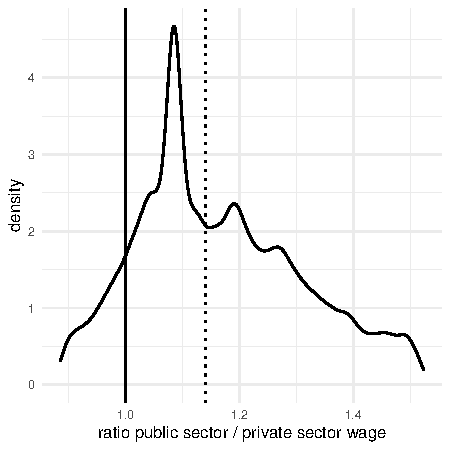
\includegraphics{chapters/chapter_2/figures/sampleDistribwwb.pdf}
    \caption{{\bf Distribution of the ratio public/private sector wage.} The dotted bar represents the median.}
    \label{fig:panel_summary}
\end{figure}

\subsection{Federal transfers and anti-corruption audits}
\label{sub:audits}

\subsubsection*{Context}

% Municipalities in Brazil rely to a large extent on federal transfers to fund their operations and payroll \citep{arretche_politicas_1999}. For some, these constitute over 90 percent of their local budget \citep{prado_transferencias_2001}. Federal transfers are designed to aid budget-constrained municipalities in achieving improvements in local public services, such as construction of new classrooms or purchase of medical supplies. Given the wide discretion conferred to municipalities as to how to manage these resources, administrative mismanagement and more serious cases of corruption are common \citep{ferraz_electoral_2007}.

Brazilian municipalities rely to a large extent on federal transfers to fund their operations and payroll \citep{arretche_politicas_1999}. For some, these constitute over 90 percent of their local budget \citep{prado_transferencias_2001}. To reduce misuse of these public resources, the Comptroller General of the Union (CGU) institutionalized in 2003 a nation-wide audits program aiming at tackling mismanagement and corruption identify irregularities in municipalities in Brazil.\footnote{For a description of the program, see \url{https://www.cgu.gov.br/assuntos/auditoria-e-fiscalizacao/programa-de-fiscalizacao-em-entes-federativos}.} Each year, a state-level lottery selects at random two municipalities per state. As such, a municipality has a 2\% chance of being audited on any given year and may be audited more than once over our period. Shortly after the lottery, teams of ten to fifteen auditors are sent to municipalities with a mandate to inspect service items and report potential irregularities in the programs that are funded through federal transfers. In our sample, auditors inspect an average of 16 items, corresponding to about \$6.8 million, or 68\% of municipal budget (Table \ref{tbl:desc}). 

Neither auditors nor the CGU have direct sanctioning power over municipalities. Irregularities are reported to the federal-level ministry responsible for the particular problematic item, and it is incumbent on that ministry to punish corruption, e.g. withholding transfers until irregularities are addressed. The CGU only has jurisdiction over the auditing of local budgets. However, audits may have direct legal consequences. Recently, the federal police, in conjunction with the CGU, began to increase efforts in cracking down on municipalities guilty of more egregious cases of corruption, such as over-invoicing or fraudulent public procurement. These special ops (\emph{operações especiais}) have led to multiple arrests of public servants found to be engaging in corruption.\footnote{See \url{http://www.cgu.gov.br/assuntos/auditoria-e-fiscalizacao/acoes-investigativas/operacoes-especiais}, for a journalistic coverage, see \url{https://g1.globo.com/pb/paraiba/noticia/2020/09/02/pf-deflagra-4a-fase-da-operacao-famintos-que-investiga-fraudes-na-merenda-em-campina-grande.ghtml}.} Similarly, the local city council may use these findings as a basis to impeach mayors.\footnote{See \url{https://g1.globo.com/sp/sao-paulo/noticia/2018/12/13/prefeito-continuou-chefiando-esquema-de-propina-em-maua-mesmo-apos-prisao-em-maio-diz-pf.ghtml}.}  %While these crackdowns may have a causal effect on dismissal rates for bureaucrats, due to data limitations they do not form part of our analysis. 

\subsubsection*{Data}

Our data reports the irregularities reported for each service order controlled by auditors from 2006 to 2015, as well as the amounts corresponding to each of these service orders. Irregularities fall into three categories: (1) notices, (2) intermediate faults, and (3) serious faults. 

We construct a series of municipal-level indicators of corruption from reported irregularities. Audits report an average of 50 intermediate faults and 8 serious faults per municipality (Table \ref{tbl:desc}). We define corruption as the \emph{intentional} abuse of public office for private gain. While our reading of reports suggest that serious faults tend to pick up corruption, we also found, in line with \citet{avis_government_2018} that the difference between intermediate and serious faults is quite blurry, as some intermediate faults also feature cases in which intentionality seems apparent, such as instances over-invoicing, shadow employees, and rigged public procurement (see Appendix \ref{app:fault} for examples). Furthermore, since larger municipalities have larger budgets, they tend to report more irregularities. 

Since there is no a priori good reason to select a particular corruption metric over another, we derive a variety of such metrics and carry our analysis over the least correlated among those. Specifically, we use, following \citet{avis_government_2018}, the count of intermediate and serious faults and the count of serious faults only. We then normalize these two metrics by the number of items audited, and also by the amount audited, for a total of 6 metrics. While many of those metrics are highly correlated, the metrics that are normalized by amount stand out (Figure \ref{fig:corruptionCorrelation} in Appendix \ref{app:fault}). We end up selecting two simple measures (\emph{all faults}, and \emph{serious faults}), and the two normalized measures that least correlate with those (\emph{all faults by amount}, and \emph{serious faults by amount}). Additionally, we de-mean irregularity counts by lottery to account for potential variation in auditing standards over time, and classify each municipality's corruption level by tercile (for more details, see Appendix \ref{app:fault}).

\subsection{Additional data}

To supplement our estimation, we collect additional data from a variety of sources. Information on electoral outcomes are gathered from the Supreme Electoral Court (TSE), containing mayor covariates such as incumbency status, age, gender and education level. 
Municipal budget from 2006 to 2015 is gathered from \textit{Finanças Brasil} (FINBRA), and demographic data from the 2001 census, collected by National Institute of Geography and Statistics (IBGE).

\section{Reduced-form estimation}
\label{sec:causal}

In this section, we ask a simple question: after an audit occurs, what happens to the careers of those bureaucrats that are currently employed in the bureaucracy? We also investigate whether audits impact managerial practices, since their improvement may indirectly curb corruption, by subjecting bureaucrats to an environment in which engaging in corruption is more difficult. We leverage the randomized nature of these audits to compare municipalities that have been audited and municipalities that have not been audited yet. Doing so, we causally identify the extent to which audits trigger waves of departures/dismissals, and improvements in managerial practices. 

We find that audits have no observable impact on career outcomes; in other words, they fail to trigger waves of departures/dismissals. This finding is surprising, given that this  program has been shown to effectively remove corrupt politicians from office \citep{ferraz_exposing_2008,ferraz_electoral_2011}, and deter them from engaging in corruption. As such, we then focus on those specific instances, and investigate whether audits trigger career interruptions for those municipalities in which we know audits have a high chance of removing the mayor from office. We fail to find evidence of such effects. We find, however, that audits lead to modest improvements in management in highly corrupt municipalities, suggesting that audits might improve the environment in which bureaucrats operate, hence reducing corruption. Overall, results therefore suggest that audits have no observable ex-post effects on bureaucratic careers and corruption. 

In what follows, we describe our approach in more details, present the results, and finally discuss how, by focusing on the observable, ex-post effects of audits, this approach is insufficient to pin down whether audits manage to curb corruption.

\subsection{Approach}
\label{sub:empiricalStrategy}

We evaluate the short-term effects of those audits on careers by estimating their average treatment effect on three outcomes: career interruptions (through dismissal or voluntary departure), and management practices. 

The effect of audits should differ depending on whether the municipality was found guilty of corruption or not. In other words, one should not expect a municipality that was not found guilty of corruption to dismiss any of its bureaucrats. As such, we gear our empirical strategy towards estimating heterogeneous treatment effects. To accomplish this, we restrict our analysis to the municipalities that have been audited over the period, because the outcome of the audit is only observable in those municipalities, and construct a time-invariant municipality \emph{type} from the result of that audit.\footnote{If municipality $j$ has been audited twice, we construct that variable using the results of the first audit.} For our estimation, we construct a trichotomous variable $c_j$ that determines whether municipality $j$ shows low, moderate, or high corruption ($c_j = 0, 1, 2$ respectively), using terciles of the distribution of corruption. 

We observe municipalities for years ranging from $\underline{t} = 2006$ to $\overline{t} = 2015$. During this period, each municipality in our sample is treated by a random anti-corruption audit at least once. Let $\tau_{jt}$ be a binary variable that equals 1 if municipality $j$ has been audited during or prior year $t$, and equals 0 otherwise. Suppose municipality $j$ was audited on year $t_j \in \{\underline{t}, ..., \overline{t}\}$. For every municipality $j$, we observe a sequence $(\tau_{j\underline{t}}, ..., \tau_{j\overline{t}})$ such that $\tau_{jt} = 0$ for any $t < t_j$ and $\tau_{jt} = 1$ for any $t \geq t_j$. We compare, within-year, our four outcomes in municipalities that have been audited to those same outcomes in municipalities that have not been audited yet, for municipalities with the same level of corruption -- low, medium, or high. With $1\{.\}$ the indicator function, our main specification reads as follows: 

\begin{equation}
    y_{jst} = \alpha_t + \alpha_s + \beta_2 \tau_{jt} + \sum_{k=1}^2 \beta_{1k} 1\{c_j = k\} +  \beta_{3k} \tau_{jt} 1\{c_j = k\} + \beta_4 x_j' + \epsilon_{jst}, 
    \label{eq:base}
\end{equation}

with $y_{jst}$ one of our three outcomes measured in municipality $j$ within state $s$ during year $t$. Therefore, $y_{jst}$ is either the log number of voluntary departures, the log number of dismissals, or a management index ranging between 0 and 1. The vector $x_j$ contains time-invariant controls; namely, the log number of employees in 2006, as well as their median wage, and the municipality-level illiteracy rate, urbanization rate and gini measured in the 2001 census, to which we add the number of audited items. Finally, $\epsilon_{jst}$ is an error term. 

The model in equation \ref{eq:base} identifies the effect of an audit on the municipality-level outcome $y_{jst}$. Parameter $\beta_2$ identifies the average treatment effect of an audit on municipalities with little corruption, while parameters $\beta_2 + \beta_{3,1}$ and $\beta_2 + \beta_{3,2}$ identify the average treatment effect of an audit on municipalities with moderate and high corruption respectively. Since audits are randomized at the state level, we include a state fixed effect $\alpha_s$ and make within-year comparisons using a year fixed effect $\alpha_t$. Additionally, we cluster standard errors at the municipality level. 

The effect of audits may present specific time dynamics. One might hypothesize that audits lead to swift waves of departures immediately after they occur or, conversely, that it takes several years to be able to dismiss tenured bureaucrats. To consider these possibility, we amend the specifications in equation \ref{eq:base} and parametrize the treatment effect flexibly. We turn our treatment indicator $\tau_{jt}$ into a categorical variable that equals to 0 prior treatment in year $t_j$, and then counts the years after treatment: $\tau_{jt} \equiv \max\{0, t - t_j + 1\}$. We therefore compare, within year, the bureaucrats that have not been audited to bureaucrats that have been audited that year, one year ago, two years ago, and so forth. 

Our last set of results shows that the electoral accountability mechanisms that we know affect politicians' careers do not trickle down to bureaucrats. To do so, we show that the hypothesis fails to pass an easy test. We focus our analysis on the cohort of bureaucrats hired by a mayor in his first term, which largely correspond to patronage appointments. If a mayor in his first term -- who therefore may run for reelection -- is found corrupt, he may have an incentive to dismiss his clients in order to wither down future electoral sanctions. Should he lose the elections, his successor also has an incentive to dismiss those bureaucrats. Intersecting these considerations is when the audits take place: presumably, audits that occur later on in the term for a first mayor, or in a more recent past for the second mayor, should have a stronger effect on bureaucratic personnel. We estimate these effects simultaneously.

We use a flexible parametrization to estimate treatment effects conditional on the political cycle. Recall that elections occur every four years. We account for a political trend that varies by municipality type using year-corruption type fixed effects. Additionally, we track, over time, the effect of having been audited on year 1, 2, 3, and 4 of the political cycle using a series of dummy variables. 

We check the robustness of our findings by conducting a series of tests, either probing the substance of the theory, or the statistical validity of the findings (results reported in Appendix \ref{app:robustness}). Regarding the substance of the theory, it might be that audits affect other segments of the bureaucracy. In other words, it might be that only a small number of key bureaucrats get dismissed. Conversely, it might be that audits trigger mass layoffs among less important employees. We show that our results extend to other categories of employees (namely, low bureaucrats, as well as high and low frontline workers, Appendix \ref{app:otherBureaucratsRobustness}), tenured and untenured bureaucrats (Appendix \ref{app:tenuredRobustness}), as well as to the most important high bureaucrats (i.e. municipal secretaries, Appendix \ref{app:secretariesRobustness}). It might also be that audits affect the composition of the pool of bureaucrats operating in the bureaucracy, and push mayors to hire more honest types. As such, we probe into hiring practices, by considering the number of hires following an audit. All other robustness checks also consider hires. We invite the reader to consult the relevant Appendix \ref{app:hiring}. % While career interruptions and management practices match the theory, we also consider hiring decisions in order to examine potential for self-selection into the bureaucracy, which was side-stepped by the model. Audits may alter hiring practices, which might alter the pool of bureaucrats. 

We also conduct tests that aim at verifying the statistical validity of the findings. We verify the randomization of audits by conducting a balance test comparing municipalities that were audited early match municipalities that were audited later on (Appendix \ref{app:balanceRobustness}). We show that our results are robust to the four corruption metrics outlined in section \ref{sub:audits}. We show that results are robust to using a measure of personnel turnover that uses percentages instead of log counts (Appendix \ref{app:percentageRobustness}), and measures of management that use only the items that occur most frequently (Appendix \ref{app:managementRobustness}). They also  We also show robustness to considering the subset of municipalities that have not been audited prior to 2006, the beginning of our period (Appendix \ref{app:neverAuditedRobustness}). Finally, we consider individual-level outcomes instead of municipal-level aggregates and show robustness to such disaggregation (Appendix \ref{app:multinomial}). 

\subsection{Results}
\label{sub:results}

Table \ref{tbl:mainMods} shows our main results, for the simplest corruption metric (total number of faults). Departure and dismissal rates for moderate- and high-corruption municipalities are indistinguishable from those of non-corrupt municipalities (columns 2 and 4). % Hiring patterns are also largely similar. There is some evidence that highly corrupt municipalities tend to hire more following an audit (model 5), but the effect disappears when introducing controls (model 6). 
Audits induce, however, significant improvements in management in highly corrupt municipalities (models 7 and 8). While audits have no effect in low and moderate corruption municipalities, they have a positive effect on the quality of management in highly corrupt municipalities ($\beta_{32} > 0$), and the overall effect of audits in high-corruption municipalities is statistically significant ($\beta_2 + \beta_{32} > 0$). The effect is, however, substantively small, with audits increasing the quality of management by 2.2 percentage points; that is, a 5\% increase relative to the sample mean. Figure \ref{fig:mainPl} shows that results extend to all the corruption metrics we consider. 

\begin{landscape}
    \begin{table}[t]
        \centering
        \footnotesize
        
% Table created by stargazer v.5.2.2 by Marek Hlavac, Harvard University. E-mail: hlavac at fas.harvard.edu
% Date and time: Sat, Sep 26, 2020 - 19:57:36
\begingroup 
\small 
\begin{tabular}{@{\extracolsep{5pt}}lcccccc} 
\\[-1.8ex]\hline 
\hline \\[-1.8ex] 
 & \multicolumn{6}{c}{\textit{Dependent variable:}} \\ 
\cline{2-7} 
\\[-1.8ex] & \multicolumn{2}{c}{No. of departures (log)} & \multicolumn{2}{c}{No. of dismissals (log)} & \multicolumn{2}{c}{Management index} \\ 
\\[-1.8ex] & (1) & (2) & (3) & (4) & (5) & (6)\\ 
\hline \\[-1.8ex] 
 Audited ($\beta_2$) & 0.134$^{*}$ & 0.068 & $-$0.075 & $-$0.111 & 0.011 & 0.0003 \\ 
  & (0.078) & (0.068) & (0.087) & (0.073) & (0.009) & (0.007) \\ 
  Moderate corruption & 0.152 & 0.123 & 0.076 & 0.090 & 0.006 & 0.004 \\ 
  & (0.107) & (0.088) & (0.111) & (0.090) & (0.011) & (0.009) \\ 
  High corruption & 0.125 & 0.039 & 0.053 & 0.070 & $-$0.008 & $-$0.020$^{*}$ \\ 
  & (0.113) & (0.104) & (0.117) & (0.108) & (0.012) & (0.011) \\ 
  Audited $\times$ Moderate corruption ($\beta_{31}$) & $-$0.134 & $-$0.104 & $-$0.001 & 0.039 & $-$0.016 & $-$0.009 \\ 
  & (0.108) & (0.095) & (0.121) & (0.102) & (0.012) & (0.010) \\ 
  Audited $\times$ High corruption ($\beta_{32}$) & 0.008 & $-$0.020 & 0.103 & 0.115 & 0.023$^{*}$ & 0.022$^{**}$ \\ 
  & (0.109) & (0.094) & (0.109) & (0.095) & (0.012) & (0.010) \\ 
 \hline \\[-1.8ex] 
Controls & \_ & \checkmark & \_ & \checkmark & \_ & \checkmark \\ 
$\beta_2 + \beta_{31}$ & 0 & -0.036 & -0.076 & -0.072 & -0.006 & -0.008 \\ 
$\beta_2 + \beta_{32}$ & 0.142 & 0.048 & 0.028 & 0.004 & 0.033*** & 0.022*** \\ 
Observations & 5,053 & 5,053 & 5,053 & 5,053 & 5,053 & 5,053 \\ 
R$^{2}$ & 0.148 & 0.300 & 0.132 & 0.269 & 0.316 & 0.441 \\ 
\hline 
\hline \\[-1.8ex] 
\textit{Note:}  & \multicolumn{6}{r}{$^{*}$p$<$0.1; $^{**}$p$<$0.05; $^{***}$p$<$0.01} \\ 
\end{tabular} 
\endgroup 

        \caption{{\bf Main results.} On average, audits have no effect on career interruptions (models 1 to 4). Audits do not decrease the number of new hires for municipalities with low and intermediate corruption either (models 5 and 6). Finally, audits are effective in improving management practices in highly corrupt municipalities (models 7 and 8). In rows $\beta_2 + \beta_{31}$, $\beta_2 + \beta_{32}$, significance stars are derived from an F-test that tests the null hypothesis $\beta_2 + \beta_. = 0$. All models include year and state fixed effects, and measure corruption using all faults. Standard errors clustered at the municipality level. See section \ref{sub:empiricalStrategy} for details about controls.}
        \label{tbl:mainMods}
    \end{table}    
\end{landscape}

\begin{figure}[h]
    \centering
    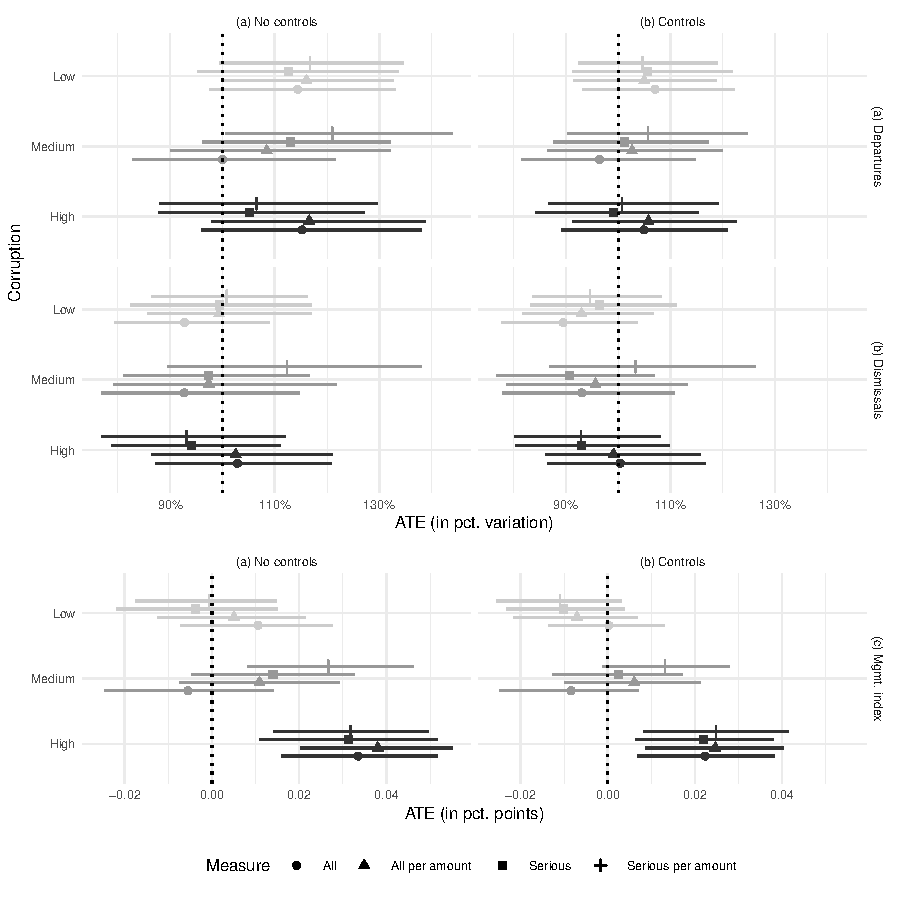
\includegraphics{chapters/chapter_2/figures/mainPl}
    \caption{{\bf Main result, different corruption metrics.} This table reestimates the specifications in Table \ref{tbl:mainMods} using all four corruption metrics. For each specification, we report the parameters $\beta_2$, $\beta_2 + \beta_{2,1}$, and $\beta_2 + \beta_{3,1}$. The top panel exponentiates these parameters to report the percentage of variation. Bars are 95 percent confidence intervals derived using semi-parametric bootstrap. Irrespective of the corruption metric, audits have a significant positive effect on the management index only for high-corruption municipalities. All other effects are not consistently significantly different from zero.}
    \label{fig:mainPl}
\end{figure}

Analyzing the effects of audits over time (Figure \ref{fig:AMEoverTime}) confirms that audits have no discernible effects on career interruptions (top two panels): for all three types of municipalities, departure and dismissal rates are comparable to pre-audit levels. Highly corrupt municipalities, however, sustain improvements in managerial practices of 0.04 percentage points immediately after an audit, with a sustained effect of 4-5 years. 

\begin{figure}[H]
    \centering
    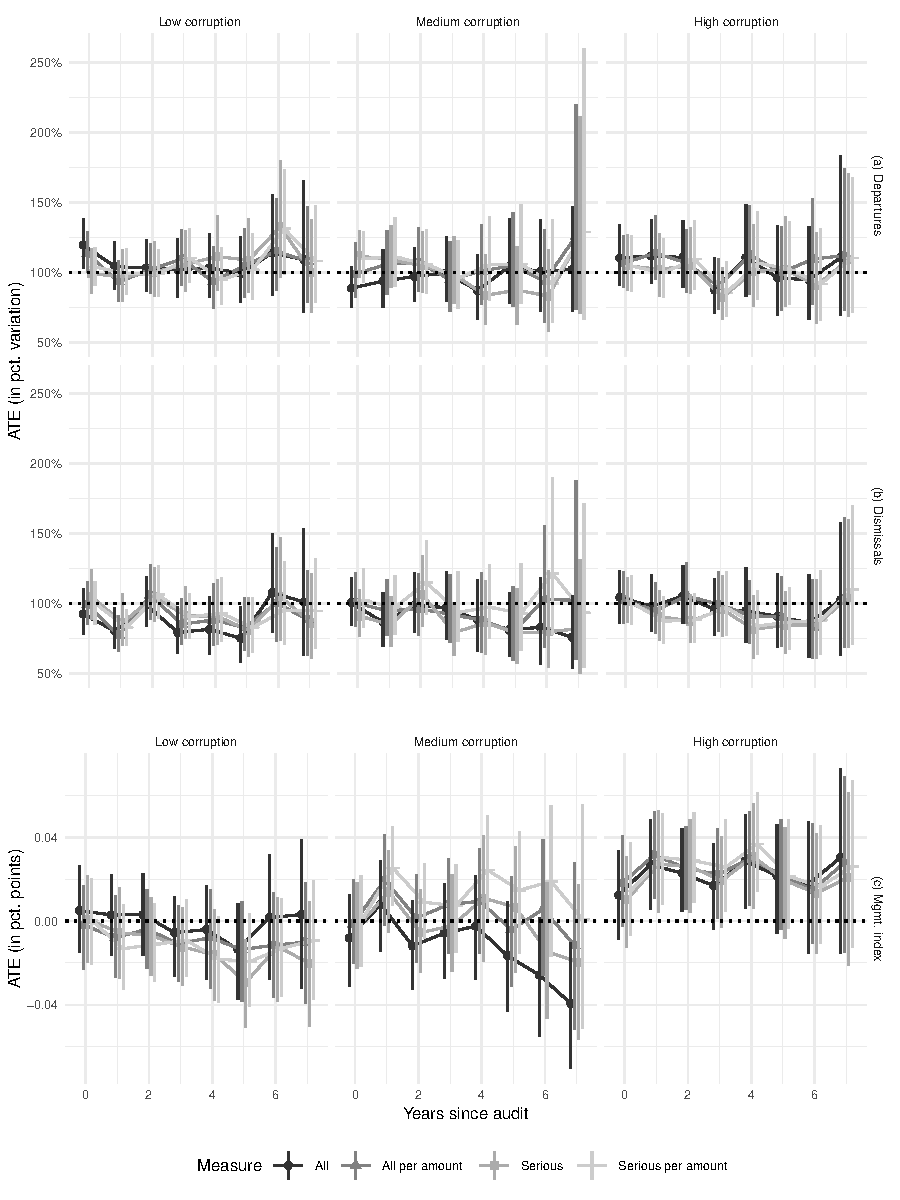
\includegraphics{chapters/chapter_2/figures/AMEoverTime}
    \caption{{\bf Treatment effect over time.} The y-axis represents the average marginal effect of some number of years after the audit on the row outcome. It is measured in percentage points for the top and bottom panels, and in percentage of variation for the middle panel. Bars are 95 percent confidence intervals clustered at the municipality level. All specifications include the controls discussed in section \ref{sub:empiricalStrategy}. Audits significantly improve management practices in high-corruption municipalities 1 to 5 years after the audit, irrespective of the corruption metric being used. All other effects are not consistently significantly different from zero.}
    \label{fig:AMEoverTime}
\end{figure}

\begin{figure}[h]
    \centering
    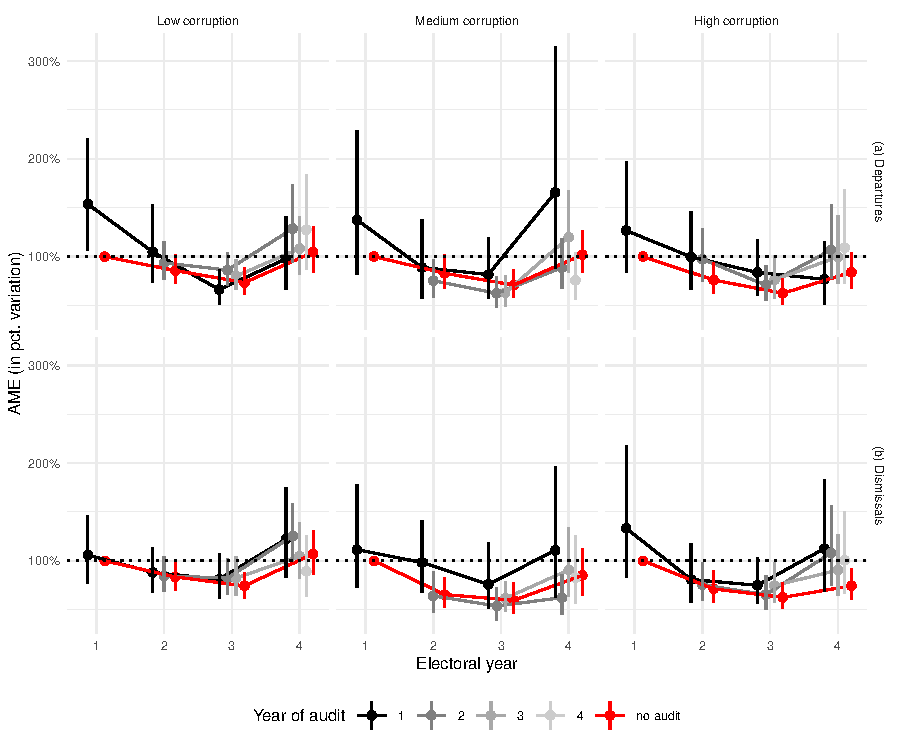
\includegraphics{chapters/chapter_2/figures/AMEpolitical_term1Client.pdf}
    \caption{{\bf Treatment effect as a function of the political cycle during the first term.} The y-axis represents the average marginal effect of audits the row outcome. The x-axis represents years in the political cycle, with year 1 being the first year of mandate. Colors indicate the year of the political cycle during which the audit occurred. Bars are 95 percent confidence intervals clustered at the municipality level. All models use the controls discussed in section \ref{sub:empiricalStrategy}. There is no evidence that audits lead to greater dismissals or departures of high-level bureaucrats.}
    \label{fig:AMEpolitical1}
\end{figure}

We finally show that electoral accountability mechanisms do not trickle down to bureaucrats. Figure \ref{fig:AMEpolitical1} reports the effects of audits during a mayor's first term, using all faults as a measure of corruption. The figure uses the first year of the electoral term as a reference category, and plots effect sizes relative to the reference category, set to the first year of term in a non-audited municipality of the type reported in the columns. As such, the red line in the top-left panel indicates variation in departures in a non-audited municipality, relative to year 1 of the term. The dark lines capture variation in departures in a municipality audited in years 1, 2, 3, and 4 of the term, again relative to relative to year 1 of the term in a non-audited municipality. While dismissals and departures do exhibit seasonality, with spikes in the first and last years of the term, audits do not significantly affect those patterns. In Appendix \ref{app:political}, we report similar effects for the subsequent mayor, and show that the findings extend to the remaining three corruption metrics. 

\subsection{Discussion}

Overall, we find that audits not trigger waves of departures or dismissals, but lead to small, temporary improvements in managerial practices. At first glance, these initial results might lead us to conclude that audits have no effect on bureaucratic careers and limited effectiveness on corruption. However, two alternative explanations are consistent with these findings and reductions in corruption. First, improvements in the quality of management might be substantial enough to trigger an \emph{unobservable, ex-post} effect; specifically, to prompt bureaucrats to temporarily switch away from dishonest behavior by making it more difficult to steal. Second, it may be that audits have \emph{disciplining} effects; in other words, they would trigger no career interruptions because even highly corrupt municipalities are not very corrupt -- recall that our measure of corruption is relative -- because the program has successfully deterred bureaucrats from engaging in corruption. This alternative would be consisted with the fact that the program is, by the end of our period, about 15 years old, giving ample time for bureaucrats to learn about the potentially severe consequences of engaging in corruption. 

Yet, our current empirical strategy makes it difficult to assess these alternative explanations. Indeed, we currently leverage the fact that audits are randomized to compare audited municipalities to municipalities that have not been audited yet. As such, the strategy may only identify \emph{ex-post, observable} effects. Probing whether audits have disciplining effects using randomization would require manipulating the \emph{threat} of an audit, and not the occurrence of audits themselves.\footnote{This approach has been explored for this program, with \citet{poulsen2019corruption} leveraging a one-time experiment in the randomization. Results suggest that these audits have indeed no significant disciplining effects, but are severely constrained by lack of power.} Similarly, with the current approach, assessing whether audits trigger temporary switches away from dishonest behavior poses a measurement problem, since it would require measuring corruption without an audit. 

We use structural estimation to circumvent these difficulties. We first develop a model that intersects bureaucratic careers with randomized audits, in order to highlight the full range of effects that these audits may have on both observable, and unobservable outcomes. We then structurally estimate the model on our data, treating corruption as a latent variable. In what follows, we first describe the model and derive a series of theoretical intuitions in simple settings, and then describe our estimation procedure and results.

\section{Theory}
\label{sec:theory}

In this section, we introduce a model that highlights all potential ways in which anti-corruption audits may impact bureaucrats' careers and reduce corruption. Indeed, our reduced-form estimates revealed that audits have no observable ex-post effects on bureaucratic careers suggesting that, at first sight, audits fail to curb corruption. Yet, our discussion highlighted a series of potential alternative explanations that would be consistent with both the observed patterns and the fact that audits do reduce corruption. This model aims at exhausting all potential channels through which audits may reduce corruption, in order to ascertain that we are not missing any. 

In the model, a bureaucrat is employed in a bureaucracy at $t = 0$ and decides on a career plan that maximizes her permanent income. At each time period, she decides whether to simply remain employed, engage in corruption, or depart to the private sector. At each time period, the bureaucracy may get audited. 

Ex-post, audits impact the agent's environment through two channels. First, with some probability, audits punish corruption that occurred in the previous period, and lead to the agent's dismissal, which we capture by a \emph{monitoring technology} parameter. The agent then joins the private sector but incurs a temporary \emph{wage penalty}, capturing a potential ``red mark'' that limits the agent's capacity to find a private-sector job. Second, audits may trigger a \emph{clean-up} of the bureaucracy that could stem, among others, from the improvements in the quality of management that we identified empirically in the previous section. Clean-ups temporarily reduce the profitability of engaging in corruption. We say that an environment in which these impacts are severe is an environment in which audits have high \emph{bite}. 

We show that, depending on how much bite they have, audits may have three kinds of consequences on bureaucrats careers and corruption. First, if audits have low bite, then they have \emph{no impact} on either careers or corruption: the bureaucrat remains in the public sector and always engages in corruption. If audits have moderate bite, they have \emph{ex-post effects}; that is, they lead to changes in behavior in response to the auditing event itself. Those include the bureaucrat getting caught for corruption and getting dismissed and, because audits may trigger improvements in management that make engaging in corruption less profitable, either temporarily refraining from corruption until the audit is over, or a departure to the private sector. Finally, if audits have high bite, they have \emph{disciplining effects}. In other words, they lead to permanent changes in behavior that reduce corruption, \emph{in anticipation} of the audits. Those include either deterring well-paid bureaucrats from stealing, or triggering preemptive departures from the bureaucracy.\footnote{This latter result, although not apparent in the simple cases we analyze in this section, becomes apparent when introducing a baseline probability of getting dismissed $q_0 \neq 0$.}

In what follows, we first describe the setting, and then derive optimal behavior under three specifications of the model. First, we examine a baseline in which audits have no bite. We then increase bite one channel at a time and allow, in turn, for audits to induce a wage penalty and to trigger clean-ups. All proofs are available in Appendix \ref{app:proofs}. We conclude by discussing what these cases tell us about the permanent and ex-post impacts of audits on careers and corruption, and discussing model assumptions. 

\subsection{Setting}

In the model, an agent is employed in a bureaucracy at $t = 0$. At each time period $t \geq 0$, she chooses an action $a_t \in \A = \{0,1,2\}$, with $a_t = 0$ corresponding to no action, $a_t = 1$ to engaging in corruption, and $a_t = 2$ to departing to the private sector, which corresponds to state $s_t = P \in \St$. Furthermore, at each time-period, the bureaucracy gets audited with probability $p$. If the bureaucracy is not audited, the agent is i{n the \emph{normal} state $s_t = N$. She is in state $s_t = A$ otherwise. As a bureaucrat, at any time-period, the agent may also get dismissed, in which case she joins the private sector, but incurs a one-period penalty (state $s_t = P'$) before joining state $P$. 

Overall, there are two occupations (public and private sector); four states ($N$ and $A$, which correspond to the public-sector occupation; and $P$ and $P'$, corresponding to the private-sector occupation); and three actions ($\A = \{0,1,2\}$). 

Transitions between states depend on the current state and actions. If the agent is in the public-sector occupation and chooses to depart, she moves to the private-sector occupation: $\Pr(s_{t+1} = P | s_t, a_t = 2) = 1$ for $s_t \in \{A, N\}$. Departures are definitive, so that $\Pr(s_{t+1} = P | s_t = P, a_t) = 1$ for any $a_t \in \A$. If she chooses to stay, she may get dismissed with baseline probability $q_0$.\footnote{Although not relevant for a theoretical exercise, this parameter improves model fit when conducting structural estimation. In the data, bureaucrats may get dismissed even in the absence of an audit. Parameter $q_0$ captures these events in a reduced form.} Additionally, if the agent is audited and stole in the previous time period, she gets detected and dismissed with probability $q$, which captures the \emph{monitoring technology} associated with audits. In other words, the agent enters the punishment state with probability $\Pr(s_{t+1} = P | s_t, a_t = 0) = q_0$ and $\Pr(s_{t+1} = P' | s_t, a_t = 1) = q_0 + (1-q_0) p q$, for $s_t \in \{A, N\}$. Since punishment lasts only one period, $\Pr(s_{t+1} = P | s_t = P', a_t) = 1$ for any $a_t \in \A$. The agent enters the normal state with probability $\Pr(s_{t+1} = N | s_t) = (1-q_0)(1-p)$ for $s_t \in \{A,N\}$, and the audited state with probability $(1-q_0)p(1-q)$.

If the agent is employed in the bureaucracy and chooses not to depart to the private sector (i.e. if $a_t \neq 2$), she earns her public sector wage $w > 0$. Additionally if she engages in corruption (i.e., if $a_t = 1$), she pockets the illegal \emph{rent} $b \geq 0$. Audits, however, may lead to a temporary \emph{clean-up} of the bureaucracy stemming, for instance, from the improvements in the quality of management we identified in the previous section. Clean-ups reduce the benefits from corruption by $c \in [0,b]$ for one period. In the private sector, in period $t$, she earns private sector wage $\wb > 0$. However, when the agent is punished, she undergoes private-sector \emph{wage penalty} $k \in [0, \wb]$. Normalizing the private-sector payoff to 0, the agent's payoff at period $t$; that is, $u : \A \times \St \rightarrow \mathbb{R}$, writes

\begin{align*}
    u(0, s_t) &= w - \wb \text{ for } s_t \in \{A,N\} \\
    u(1, N) &= b + w - \wb \\
    u(1, A) &= b - c + w - \wb \\ 
    u(a_t, P) &= 0 \text{ for any } a_t \in \A \\
    u(a_t, P') &= - k \text{ for any } a_t \in \A
\end{align*}

The agent is infinitely-lived, discounts the future with rate $\de \in (0,1)$, and maximizes her permanent income. In other words, she chooses a policy $\pi : \St \rightarrow \A$, which maps states $s_t$ to actions $a_t$.\footnote{Since payoffs $u$ are bounded and stationary, and transition probabilities are also stationary, and $\St$ and $\A$ are finite, a stationary policy $\pi : \St \rightarrow \A$ is optimal.} With $\Pi$ denoting the set of possible policies, our agent solves the following dynamic programming problem 

$$
\max_{\pi \in \Pi} \mathbb{E} \left[ (1-\de) \sum_{t = 0}^\infty \delta^t u(\pi(s_t), s_t) \right] 
$$

for initial state $s_0 \in \{A,N\}$. 

In what follows, we solve this problem under a few additional assumptions that we will relax when estimating the model structurally.\footnote{Specifically, the structural model makes no additional assumptions on $q_0, k, c$.} Throughout the section, we assume that the baseline probability of dismissal $q_0 = 0$. Additionally, how public and private sector wages compare has important implications. There are three possible cases:

\begin{align}
    w < w+b < \wb \label{eq:wi} \\ 
    w < \wb < w+b \label{eq:wwb} \\
    \wb < w < w+b \label{eq:wbw}
\end{align}
Case \ref{eq:wi} is not interesting in the context of this model, because departing to the private sector dominates both honest and corrupt behavior. In case \ref{eq:wwb}, bureaucrats are underpaid relative to the private sector, but corruption is more profitable than private-sector employment. In case \ref{eq:wbw} on the other hand, bureaucrats are overpaid relative to the private sector. 

We start by analyzing the simplest model, setting $k = c = 0$. We then examine how introducing a wage penalty changes the results, and analyze the case in which $k > 0$, $c = 0$. We finally examine how introducing clean-ups affects the results, focusing on the case in which $k = 0$, $c > 0$. 

\subsection{A baseline model}

We first analyze the case where $k = c = 0$. Note that in this case, states $A$ and $N$ are payoff-equivalent, and so are states $P$ and $P'$. As such, we only need consider policies in which the agent steals in both states ($\pi(N)=\pi(A)=1$), in neither state ($\pi(N)=\pi(A)=0$), or quits preemptively ($\pi(N)=\pi(A)=2$). 

When $w < \wb < w+b$, the only reason to stay in the public sector is to pocket rents. Since engaging in corruption is more profitable than quitting and incurs no penalty, it is optimal for the agent to steal in every period until she gets dismissed. When $\wb < w < w+b$, the agent would rather stay in the public sector than depart to the private sector. As such, if corruption is very profitable (i.e. if $b$ is large enough), then the expected benefits from corruption are higher than the risk of joining the private sector, and stealing is optimal. Conversely, when corruption is not profitable enough, not stealing is optimal (see Figure \ref{fig:eq0} for an illustration). Formally: 

\begin{proposition}
    \label{prop:eq0}
    If $k = c = 0$, then $\pi^*(N)=\pi^*(A)=1$ is optimal if equation \ref{eq:wwb} holds. If equation \ref{eq:wbw} holds, then there is $b_0 > 0$ such that $\pi^*(N)=\pi^*(A)=0$ is optimal whenever $b \leq b_0$, and $\pi^*(N)=\pi^*(A)=1$ is optimal whenever $b \geq b_0$. Other stationary policies are not optimal. 
\end{proposition}

\begin{figure}[H]
    \centering
    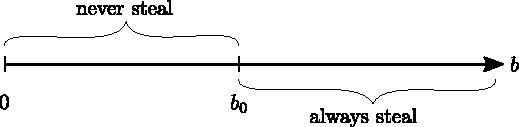
\includegraphics{chapters/chapter_2/figures_theory/eq_baseline.pdf}
    \caption{{\bf Graphical illustration of proposition \ref{prop:eq0} in the case where $\wb < w < w+b$.} The strategies ``always steal'' and ``never steal'' correspond, respectively, to $\pi(N) = \pi(A) = 1$ and $\pi(N) = \pi(A) = 0$.}
    \label{fig:eq0}
\end{figure}

\subsection{Introducing a wage penalty}

We now consider the case where $k > 0$ and $c = 0$. Compared to the baseline, states $A$ and $N$ are still payoff-equivalent, but states $P$ and $P'$ are not. Here engaging in corruption carries the additional cost of a one-time wage penalty $k$ after being dismissed. 

When $w < \wb < w+b$, then stealing is always optimal. The only reason why the agent would switch to its second most attractive policy -- that is, quitting preemptively -- is because the penalty from stealing $k$ is too high. Yet, such deterrence would require a disproportionately high outside option, i.e. it would require $\wb \gg w+b$. 

When $\wb < w < w+b$, then 
\begin{proposition}
    \label{prop:eqK}
    If $k > 0$ and $c = 0$, then there is $k_0$ such that $\pi^*(N)=\pi^*(A)=1$ is optimal whenever $k \leq k_0$, and $\pi^*(N)=\pi^*(A)=0$ is optimal whenever $k \geq k_0$. If equation \ref{eq:wwb} holds, then $k_0 > \wb$. If equation \ref{eq:wbw} holds, then there are $b_0, b_1$ with $0 < b_0 < b_1$ such that $k_0 < 0$ if $b < b_0$, $k_0 \in [0,\wb]$ if $b \in [b_0, b_1]$, and $k_0 > \wb$ otherwise. Other stationary policies are not optimal. 
\end{proposition}
Proposition \ref{prop:eqK}, illustrated graphically in Figure \ref{fig:eqK}, tells us that if the wage penalty is sufficiently high, it has a deterrence effect, pushing agents to never steal. Conversely, it if is not high enough, then the agent engages in corruption until she gets detected and punished. Again, since $w < \wb < w+b$, never stealing is not attractive. 

\begin{figure}[H]
    \centering
    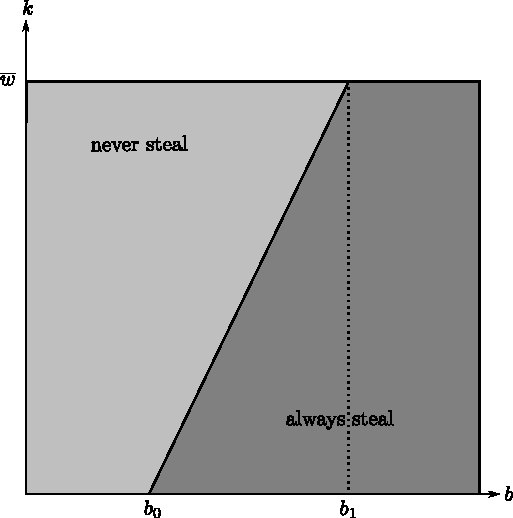
\includegraphics{chapters/chapter_2/figures_theory/eq_with_k.pdf}
    \caption{{\bf Graphical illustration of proposition \ref{prop:eqK} in the case where $\wb < w < w+b$.} The strategies ``always steal'' and ``never steal'' correspond, respectively, to $\pi(N) = \pi(A) = 1$ and $\pi(N) = \pi(A) = 0$.}
    \label{fig:eqK}
\end{figure}

\subsection{Introducing a clean-up effect}

We finally consider the case where $k = 0$ and $c > 0$. Compared to the baseline, states $P$ and $P'$ are still payoff-equivalent, but states $A$ and $N$ are not. Here, audits trigger a temporary clean-up of the bureaucracy, which make engaging in corruption less profitable after an audit. 

When $w < \wb < w+b$ (Figure \ref{fig:eqC}, left panel), always stealing is optimal if the clean-up is sufficiently small. When such clean-up effect increases and makes rents too small, other policies become optimal. Which policy is optimal depends on the size of the benefit $b$. If both $b$ and $c$ are large, then the agent has an incentive to refrain from stealing for the one period during which the clean-up effect lasts (i.e. $\pi(A) = 0$), and resume afterwards (i.e. $\pi(N) = 1$). When $b$ is small, increases in $c$ make corruption less profitable overall, and agents retrench to the private sector after the first audit (i.e. $\pi(A) = 2$). 

\begin{figure}[H]
    \centering
    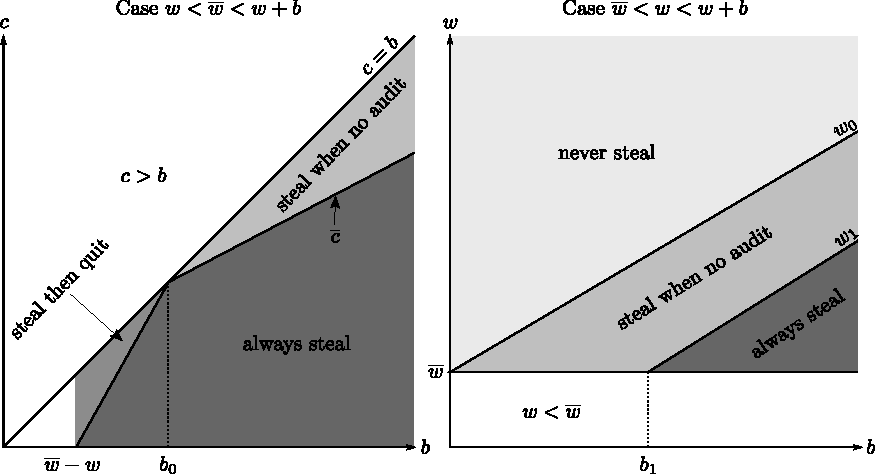
\includegraphics{chapters/chapter_2/figures_theory/eq_with_c.pdf}
    \caption{{\bf Graphical illustration of proposition \ref{prop:eqC}.} The policies ``never steal,'' ``always steal,'' ``steal when no audit,'' and ``steal then quit'' correspond, respectively, to $\pi(A) = \pi(N) = 0$; $\pi(A) = \pi(N) = 1$; $\pi(A) = 0, \pi(N) = 1$;  and $\pi(A) = 2, \pi(N) = 1$.}
    \label{fig:eqC}
\end{figure}

When $\wb < w < w+b$ (Figure \ref{fig:eqC}, right panel), always stealing is optimal if $w$ is sufficiently small and $b$ sufficiently large to both offset the clean-up effect and the risk of being dismissed to the less attractive private sector. As $w$ increases and $b$ decreases, agents first revert to only stealing after the clean-up has worn off. As $w$ further increases and $b$ further decreases, engaging in corruption is not worth the risk, so agents refrain from stealing. Formally:  

\begin{proposition}
    \label{prop:eqC}
    Suppose $k = 0$ and $c > 0$. If equation \ref{eq:wwb} holds, then there is $\overline{c}(b) \leq b$ such that $\pi^*(N)=\pi^*(A)=1$ is optimal whenever $c \leq \overline{c}$. The policy $\pi^*(N)=1, \pi^*(A)=2$ is optimal whenever $c \geq \overline{c}$ and $b \leq b_0$ such that $w+b_0 \geq \wb$. Finally, the policy $\pi^*(N)=1, \pi^*(A)=0$ is optimal whenever $c \geq \overline{c}$ and $b \geq b_0$. If equation \ref{eq:wbw} holds, then the policy $\pi^*(N)=\pi^*(A)=0$ is optimal whenever $w \geq w_0 \geq \wb$. The policy $\pi^*(N)=1, \pi^*(A)=0$ is optimal whenever $w \in [w_0,w_1]$, with $w_1 \geq \wb \iff b \geq b_1 > 0$. Finally, the policy $\pi^*(N)=\pi^*(A)=1$ is optimal whenever $w \leq w_1$ and $b \geq b_1$. Other stationary policies are not optimal. 
\end{proposition}

\subsection{Discussion} 

The model tells us that audits affect bureaucrats' careers through multiple channels. A useful way to categorize these effects is to separate them according to (1) personnel's behavior: whether bureaucrats depart the bureaucracy, get dismissed, or simply refrain from corruption while remaining employed, and (2) the timing of those effects: whether agents alter their behavior ex-ante, i.e. disciplining effects, or after the audit occurs, i.e. ex-post effects. 

Audits may have disciplining effects, which occur when audits have high bite; that is, when $k, c$, or $q$ are high. Immediately, they may permanently deter corruption because the risk of getting dismissed and forced to join the private sector -- perhaps compounded with ensuing wage penalties -- outweighs the benefit. Such effect, however, requires that public sector wages be higher than private sector wages. Another disciplining effect, not seen in the above discussion, becomes apparent when considering a non-zero baseline probability of dismissal (i.e. $q_0 > 0$): audits trigger preemptive waves of departures.  

As the bite of audits decreases, audits move from disciplining to ex-post effects. The most obvious such effects is the dismissal of employees that engage in corruption. Moreover, bureaucratic clean-ups immediately after an audit can prompt additional effects. Specifically, for those bureaucrats for whom the private sector is a poor option, while large improvements trigger permanent effects, smaller improvements push those bureaucrats to refrain from stealing temporarily. Clean-ups also have ex-post effects on those bureaucrats for whom the private sector is attractive: they steal until the clean-up occurs and then leave.

If audits are ineffective, then bureaucrats simply engage in corruption throughout their careers, and get dismissed if they ever get caught. In the context of our model, audits can fail to induce observable changes in bureaucratic behavior because they have little bite: $c$, $q$ or $k$ are too small to deter bureaucrats from always stealing. 

This model makes a series of stark assumptions. Specifically, (1) we abstract away from a series of well-known determinants of individual bureaucratic behavior, especially as far as corruption is concerned, and (2) we consider an individual bureaucrat in isolation. Regarding the first point, the model does not explicitly feature public sector motivation \citep{dal2013strengthening}, nor moral costs of corruption \citep[see e.g.][]{roseackerman1975}. These dimensions can, however, be easily integrated in the model by interpreting parameters $b$ and $w$ as reduced-forms. Specifically, parameter $w$ could incorporate both a monetary wage, as well as a latent public sector motivation. Conversely, parameter $b$ could incorporate both a (positive) monetary reward from corruption and a (negative) moral cost of corruption. In this setting, it may then be that, contra model assumptions, $b \leq 0$. In this case, the model becomes trivial: agents have no incentive to engage in corruption; they simply compare their public- and private-sector wages, and join the occupation that is most rewarding. 

The second point, namely that the model considers an individual bureaucrat in isolation, is a simplifying choice. The setting does not explicitly feature other bureaucrats, nor a political principal. A more realistic model would have a political principal and other bureaucrats affect parameters $b, c, q$. More bureaucrats engaging in corruption may, for instance, impose externalities on the size of rents $b$, either reducing them (e.g. through crowding-out effects), or increasing them (e.g. through cooperation; see \citet{shleifervishny1993corruption} for a discussion of when either effect could materialize). Similarly, the political principal may engage in corruption herself, hence adopting lenient responses, and setting $c$ and $q$ to low values, or instead be tough on corruption, hence setting $c$ and $q$ to high values (see e.g. \citet{ferraz_electoral_2011} for a discussion of when each of these may occur). We interpret our results as partial equilibrium results in which we explore the full range of parameter values for $b,c$ and $q$. Doing so is in the spirit of the exercise, whose goal is to explore the full range of effects that audits may have. In other words, moving the model from decision theory to game theory by introducing additional players would eliminate some of the solutions we characterized above. 

\section{Structural estimation}
\label{sec:structural}

Having devised a model that shows all the ways in which audits may affect bureaucratic careers and corruption, we use it to guide a more informed exploration of the data. Full structural estimation of the model is challenging, for two reasons: first, we do not observe whether agents engage in corruption or not (i.e., whether $a_{it} = 0$ or 1) and second, the model attributes all the part of the decision to stay that cannot be attributed to the wage differential $w - \wb$ to rents from corruption $b$, ignoring the well-known fact that bureaucrats may derive non-monetary benefits from staying in office, which we broadly refer to as public sector motivation. These two points make identifying a structural model challenging, because it is unclear whether the low dismissal and departure rates observed in the data owe to high corruption, high rents and low probability of sanction, or lack of corruption because of a large threat of punishment. 

Given these difficulties, we chose an intermediate approach and estimate a dynamic discrete choice (DDC) model. This model moves closer to the theory by introducing forward-looking agents and payoff functions that resemble the theory. It differs from the theory by lumping the decision of engaging in corruption or not into a decision of staying in the bureaucracy. Using the results from audits as proxies for municipal-level corruption, parameter estimates average over agents that steal and agents that do not. They separate for agents with observed characteristics $x_i$ (1) an average level of rents that varies systematically according to observed municipal levels of corruption -- presumably capturing illegal rents, (2) an average short-term effect of those audits on such rents, and (3) a time- and municipality-invariant rent that may owe to public sector motivation or unobserved rents. 

In what follows, we first describe the DDC model and present our results. The results rule out unobservable ex-post effects and any systematic variation in the size of rents according to observed levels of municipal corruption. The results show that bureaucrats remain in office much more than what would be expected given their public/private-sector wage differential, leaving us with two opposite conclusions as to the effectiveness of the program: either the program has a strong disciplining effect and bureaucrats' stickiness owes to strong public sector motivation, or it has a weak disciplining effect and bureaucrats stay in office because they pocket large rents from corruption. We finally use those estimates to calibrate a series of counterfactual experiments that investigate ways of making the program more effective. 

\subsection{Approach}
\label{sub:approachStructural}

In this model, bureaucrat $i$ in municipality $j$ makes at each period $t$ the career decision $y_{ijt} \in \{0,1\}$, with 0 corresponding to staying in the public sector, and 1 to departing to the private sector. The crucial differences between this model and the theoretical model is that now, the agent gets payoff $b_{ij}$ from engaging in corruption that does not depend upon her actions, and enjoys (non-monetary) public sector motivation $m_i$. Additionally, at each time period, and for every potential choice, the agent enjoys taste shock $\epsilon^y_{ijt}$ Normalizing to 0 her payoff in state $P$, the agent's flow payoff writes: 
\begin{align*}
    u_{ijt}(0, N) &= b_{ij} + m_i + w_i - \wb_i + \epsilon^0_{ijt} \\ 
    u_{ijt}(0, A) &= b_{ij} - c_i + m_i + w_i - \wb_i + \epsilon^0_{ijt} \\ 
    u_{ijt}(1, N) &= u_{ijt}(1, A) = u_{ijt}(y_{it}, P) = 0 + \epsilon^y_{ijt} \\ 
    u_{ijt}(y_{it}, P') &= -k_i + \epsilon^y_{ijt}
\end{align*}
If the agent choses to stay in the public sector, she gets dismissed with probability $q^A_j$ and $q^N_j$ in the respective events that the bureaucracy gets audited or does not. The transition matrix for $y_{ijt} = 1$ has $\Pr(s_{ijt+1} = P | y_{ijt} = 1, s_{ijt}) = 1$ for any $s_{ijt}$. The transition matrix for $y_{ijt} = 0$ writes

$$
\kbordermatrix{
    & N & A & P' & P  \\
    N & (1-p)(1-q^N_j) & p(1-q^A_j) & (1-p)q^N_j + p q^A_j & 0 \\
    A & (1-p)(1-q^N_j) & p(1-q^A_j) & (1-p)q^N_j + p q^A_j & 0 \\
    P' & 0 & 0 & 0 & 1  \\
    P & 0 & 0 & 0 & 1 
  }
$$

We assume that $b_{ij}$ is a function of observed, municipal level corruption $\bb_j$, a vector of individual-level time-invariant characteristics $x_i$; i.e. $b_{ij} = f(\bb_j, x_i)$. We assume that $m_i$ are $c_i$ are also functions of $x_i$; i.e. $m_i = g(x_i)$ and $c_i = h(x_i)$. Let's assume, finally, that $f$, $g$ and $h$ are linear functions: $f(\bb_j, x_i) = \alpha_b + \bb_j \beta_b + x_i' \bb_j \gamma_b$, $g(x_i) = \alpha_m + x_i' \beta_m$ and $h(x_i) = \alpha_c + x_i' \beta_c$. The agent's flow payoff from action 0 in states $A$ and $N$ writes 

$$
    u_{ijt}(0, s \in \{A, N\}) = \alpha_m + \alpha_b + x_i' \beta_m + \bb_j \beta_b + x_i' \bb_j \gamma_b - 1\{s = A\} \left[\alpha_c + x_i' \beta_c \right] + w_i - \wb_i + \epsilon^0_{ijt}
$$

The agent makes decisions that maximize its long-run discounted payoff
$$
U(y_{ij0}, y_{ij1}, \dots) = \mathbb{E} \left\{ \sum_{t=0}^\infty \delta_i^t u_{ijt}(y_{ijt}, s_{jt}) \right\}
$$

We estimate this model, up to parameters $\alpha_m$ and $\alpha_b$, using the two-step conditional choice probability partial likelihood estimator \citep{hotzmiller1993ccp} and a series of auxiliary models. We observe the states, career decisions, as well as characteristics $x_i$ that include gender, level of education and contract type. We estimate $w_i$, $\wb_i$, $\delta_i$, $k_i$ using auxiliary models that we detail in Appendix \ref{app:structural}. We estimate state transition probabilities $q^A$, $q^N$ non-parametrically. We obtain first-stage estimates of conditional choice probabilities using a logistic regression with municipal-level fixed effects, controlling for $x_i$ and the state. We then use those state transition probabilities and conditional choice probabilities to derive estimates of the conditional value function and finally estimate parameters $\beta_m, \beta_b, \gamma_b, \alpha_c, \beta_c$ and parameter $\theta = \alpha_m + \alpha_b$ in a second-stage logistic regression. 

Note that the model is fully identified under the assumption that $f(0) = 0$; that is, assuming that in municipalities in which audits reveal no corruption have indeed no corruption. Indeed, the assumption implies that $\alpha_b = 0$, and therefore that $\theta = \alpha_m$. In that case, we get $\theta + x_i' \beta_m = m_i$, $\bb_j \beta_b + x_i' \bb_j \gamma_b = b_i$ and $c_i = \alpha_c + x_i' \beta_c$. 

We shy away from making this arguably strong assumption. Our estimates therefore recover the short-term change in such rents following audits $c_i$, the part of rents from corruption that varies with municipal corruption and individual characteristics, i.e. $b_{ij} - \alpha_b$, and the part of public sector motivation that varies with individual-level characteristics, i.e. $m_i - \alpha_m$. The intercept $\theta$ conflates a baseline level of public sector motivation and a baseline level of rents from corruption. 

\subsection{Estimates, validation and counterfactual experiments}

\begin{table}[h]
    \centering
    
% Table created by stargazer v.5.2.2 by Marek Hlavac, Harvard University. E-mail: hlavac at fas.harvard.edu
% Date and time: Fri, Jan 08, 2021 - 2:22:12 PM
\begingroup 
\footnotesize 
\begin{tabular}{@{\extracolsep{5pt}}lc} 
\\[-1.8ex]\hline 
\hline \\[-1.8ex] 
 Constant ($\theta = \alpha_m + \alpha_b$) & 1.985$^{***}$ \\ 
  & (0.297) \\ 
  education - 2ary ($\beta_{m1}$) & $-$0.074 \\ 
  & (0.196) \\ 
  education - higher ($\beta_{m2}$) & $-$0.742$^{***}$ \\ 
  & (0.174) \\ 
  male ($\beta_{m3}$) & $-$0.209$^{***}$ \\ 
  & (0.074) \\ 
  tenure ($\beta_{m4}$) & 0.363 \\ 
  & (0.272) \\ 
  $\overline{b}_j$ ($\beta_b)$ & 0.020 \\ 
  & (0.020) \\ 
  $\overline{b}_j \times$ education - 2ary ($\gamma_{b1}$) & 0.009 \\ 
  & (0.016) \\ 
  $\overline{b}_j \times$ education - higher ($\gamma_{b2}$) & 0.009 \\ 
  & (0.012) \\ 
  $\overline{b}_j \times$ male ($\gamma_{b3}$) & $-$0.006 \\ 
  & (0.005) \\ 
  $\overline{b}_j \times$ tenure ($\gamma_{b4}$) & $-$0.007 \\ 
  & (0.019) \\ 
  audit $\times$ education - 2ary ($\beta_{c1}$) & 0.107 \\ 
  & (0.219) \\ 
  audit ($\alpha_c$) & $-$0.006 \\ 
  & (0.128) \\ 
  audit $\times$ education - higher ($\beta_{c2}$) & 0.159 \\ 
  & (0.168) \\ 
  audit $\times$ male ($\beta_{c3}$) & 0.039 \\ 
  & (0.062) \\ 
  audit $\times$ tenure ($\beta_{c4}$) & $-$0.220 \\ 
  & (0.254) \\ 
 \hline \\[-1.8ex] 
Observations & 671,831 \\ 
\hline 
\hline \\[-1.8ex] 
\textit{Note:}  & \multicolumn{1}{r}{$^{*}$p$<$0.1; $^{**}$p$<$0.05; $^{***}$p$<$0.01} \\ 
\end{tabular} 
\endgroup 

    \caption{{\bf Standardized DDC estimates.} The intercept $\theta = \alpha_m + \alpha_b$ is large, while the part of rents from corruption that varies with municipal corruption and individual-level characteristics ($b_{ij} - \alpha_b$) is small and not significantly different from zero, and so is the clean-up effect $c_i$. Standard errors are clustered at the municipal level and obtained through a non-parametric bootstrap procedure with 10,000 replicates.}
    \label{tbl:strut_results}
\end{table}

Table \ref{tbl:strut_results} reports standardized parameter estimates from our DDC model. We see that the intercept $\theta = \alpha_m + \alpha_b$ is large, while the part of rents from corruption that varies with municipal corruption and individual-level characteristics (i.e. parameter $\beta_b$) is small and not significantly different from zero, and so is the parameter $\beta_c$ on the clean-up effect $c_i$. 

\begin{figure}[h]
    \centering
    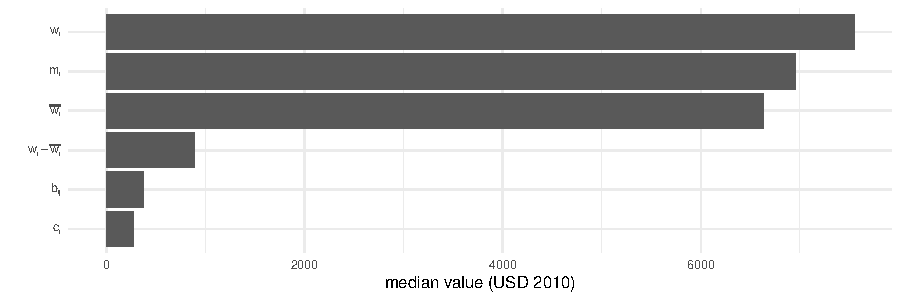
\includegraphics{chapters/chapter_2/figures/distribStructural.pdf}
    \caption{{\bf Median values of quantities of interest.} This figure reports the median in-sample value of quantities of interest under the assumption that $\alpha_b = 0$. We see that public sector motivation $m_i$ is large, amounting to about 90\% of median wage $w_i$. Rents from corruption $b_{ij}$ and the clean-up effect $c_i$ are small.}
    \label{fig:mainResultStructural}
\end{figure}

Figure \ref{fig:mainResultStructural} reports the unstandardized, median in-sample value of quantities of interest under the assumption that $\alpha_b = 0$ (i.e. that the intercept only captures public sector motivation). We find that public sector motivation $m_i$ is large, amounting to about 90\% of median wage $w_i$. Rents from corruption $b_{ij}$ and the clean-up effect $c_i$ are small. 

Together these results show that (1) departure rates show systematic little variation across municipalities as a function of the number of irregularities reported by audits; (2) they also show little variation depending on whether the municipality is audited or not; and (3) that the public/private-sector wage differential $w_i - \wb_i$ is insufficient to account for the low departure rates observed in the data. While results (1) and (2) echo our reduced-form results on the number of departures, result (3) adds an important detail to the picture: bureaucrats' stickiness owes to a large unobserved component $\theta$. Whether that component captures an invariant payoff from public sector motivation $\alpha_m$ or invariant rents from corruption $\alpha_b$ is an open question. 

These results are consistent with two opposite conclusions as to the effectiveness of the audits program; namely that the program either has a large or a small disciplining effect. Our reduced-form estimates showed that the ex-post, observable effect of the program is small. Structural estimates established that the ex-post, unobservable effect of the program is also small. Whether the program has a disciplining effect is an open question. If $\theta$ mostly captures public sector motivation, then the program has a large disciplining effect. Under this hypothesis, rents from corruption are negligible while public sector motivation is large. The low dismissal and departure rates observed in the data indicate that bureaucrats stay in office because they derive large public sector motivation, as the program has successfully eliminated corrupt rents. Conversely, if $\theta$ mostly captures rents from corruption, then the program also has a negligible disciplining effect. Under this hypothesis, rents from corruption are large while public sector motivation is negligible. The low dismissal and departure rates observed in the data indicate that bureaucrats stay in office because they derive large rents from corruption, and that the program is unable to remove corrupt bureaucrats from office.

We validate these estimates by checking that they match patterns observed in the data. We check whether the career paths implied by estimated parameter values match the career paths observed in the data (Appendix \ref{app:structural}, Figure \label{fig:validationStructuralSize}). To do so, we compare year to year variation in the size of the bureaucracy as observed in the data to predicted variation under parameter values. We find that our predictions match the data remarkably well, except for years 2008 and 2012, where we fail to predict the large waves of departures and dismissals. As discussed in section \ref{sec:causal}, these years are pre-electoral years, during which turnover is large, a feature that we did not include in the model.  

We finally evaluate the impact of the program by comparing the total amount of rents extracted through corruption to a series of counterfactual benchmarks under the theoretical model analyzed in section \ref{sec:theory}, in which we augment flow payoffs with random extreme value type I shocks. This computational exercise is calibrated using parameter estimates from the DDC model. Doing so amounts to ascribing the average effects identified by the DDC model to structural parameter values. The assumption would be verified under the admittedly unrealistic case in which all agents always engage in corruption.  Should some agents not engage in corruption, then the assumption understates gains from corruption $b$, the clean-up effect $c$, and the probability of dismissal $q$. Furthermore, since, as argued above, it is unclear whether the intercept $\theta$ captures public sector motivation or invariant rents from corruption, we consider the following three scenarios: (1) $\theta = \alpha_m$, (2) $\theta = \frac{\alpha_m}{2} + \frac{\alpha_b}{2}$, and (3) $\theta = \alpha_b$. In other words, we assume that the intercept either fully captures public sector motivation (case 1), fully captures invariant rents from corruption (case 3), or is composed in equal parts of public sector motivation and rents from corruption (case 2). 

We consider a \emph{baseline}, which corresponds to predictions under the estimated parameters. We compare this baseline against two benchmarks. First, a \emph{negative benchmark} in which we set both $c$ and $q$ to zero. This allows evaluating how much corruption has been deterred by the program, compared to a counterfactual in which the program was never enacted. We then compare our baseline to a \emph{positive benchmark}, in which we set again both $c$ and $q$ to zero, but reduce the size of rents to the median for all those municipalities for which $b$ is above the median. This positive benchmark corresponds to a counterfactual world in which audits never took place, but the size of rents is halved. All scenarios consider the distribution of states as they occurred in the data (i.e. we use the realizations of audits that occurred in the data). They consider each sample bureaucrat on the year they enter the sample and estimate their optimal policy given parameter values. This allows deriving their probability of departure/dismissal, and expected amount stolen over the period. Aggregating to the sample level allows deriving the predicted size of the bureaucracy, cumulative amount stolen, and policy distribution with respect to expected behavior.

Comparing the baseline to the negative benchmark in which we remove audits (Figure \ref{fig:counterfactuals1}), we find that the program had little impact on corruption: irrespective of the assumption on $\theta$, the program reduced corruption by less than 2 percentage points. Comparing the baseline to the positive benchmark confirms the finding. Halving the size of rents reduces total corruption by 75, 17, or 9 percentage points depending on whether $\theta$ fully captures public sector motivation, a mix of public sector motivation and corruption, or fully captures corruption respectively.  


% We also consider both mechanisms in isolation by setting each parameter separately (i.e., a ``$c$'' and a ``$q$'' scenario). Finally, we consider a scenario that decreases the size of the rent $b$. We interpret $b$ as an indicator of the broader institutional environment in which bureaucrats evolves, that in fine impacts the size of potential gains from corruption. We consider $b$ relative to the municipality's mean public sector wage $\tilde{w}$, and set to the 5th percentile in the distribution of $b_j/\tilde{w}_j$ all municipalities above the 5th percentile.  All scenarios consider each sample bureaucrat on the year they enter the sample and estimate their optimal policy given parameter values. This allows us to derive their probability of departure, and expected amount stolen over the period. Aggregating to the sample level allows deriving the predicted size of the bureaucracy, cumulative amount stolen, and policy distribution with respect to expected behavior.

\begin{figure}[H]
    \centering
    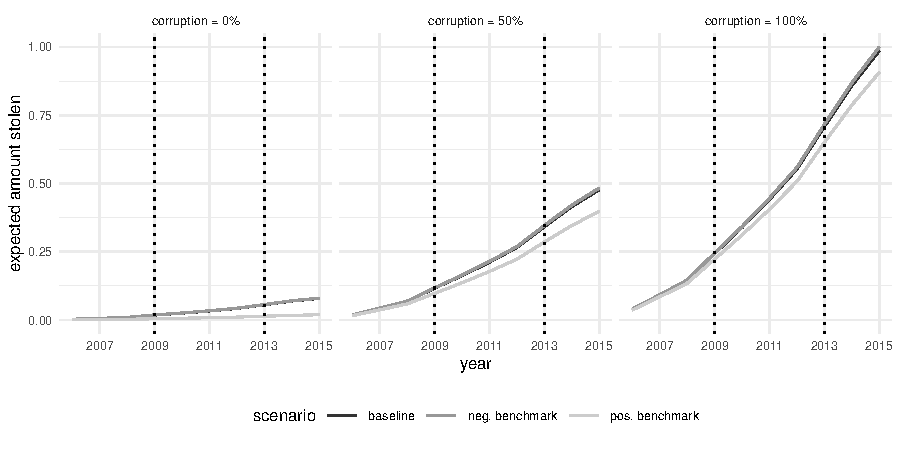
\includegraphics{chapters/chapter_2/figures/counterfactuals1.pdf}
    \caption{{\bf Impact of the program on corruption.} The program occasioned less that a 2 percentage points decrease in overall corruption comparing to a benchmark in which audits never occurred. This is a far cry from halving the size of the rents (positive benchmark), which reduces the amount of corruption by about 75, 17, or 9 percentage points (left to right panel).}
    \label{fig:counterfactuals1}
\end{figure}

We finally investigate ways to make the program more effective. To do so, we construct a series of counterfactuals in which we progressively increase the value of each of the parameters $p, c, q$ from 0 to 1 for all those municipalities which fall below the target value, while keeping other parameters constant. We finally consider a scenario which increase all three parameters jointly. We examine, for each of these scenarios, the total expected amount stolen by the end of the period. Our key comparison is how much reduction in corruption those scenarios achieve compared to the baseline, and our positive benchmark. 

The results, reported in Figure \ref{fig:counterfactuals2}, show that, considering each component of the program in isolation, increasing the strength of monitoring associated with  audits (i.e. parameter $q$) is the most effective way of reducing corruption. If corruption was met with certain dismissal (recall that the average $q = 0\%$), corruption would decrease by 25, 15, and 12 percentage points depending on whether $\theta$ fully captures public sector motivation, a mix of public sector motivation and corruption, or fully captures corruption respectively. This, however, only matches our positive benchmark in the latter two cases. The most effective way to reduce corruption is to increase all parameters jointly, suggesting that program components display strong complementarities. Irrespective of the hypothesis on $\theta$, increasing all parameters to 25\% is more effective than punishing corruption with certain dismissal. 

\begin{figure}[H]
    \centering
    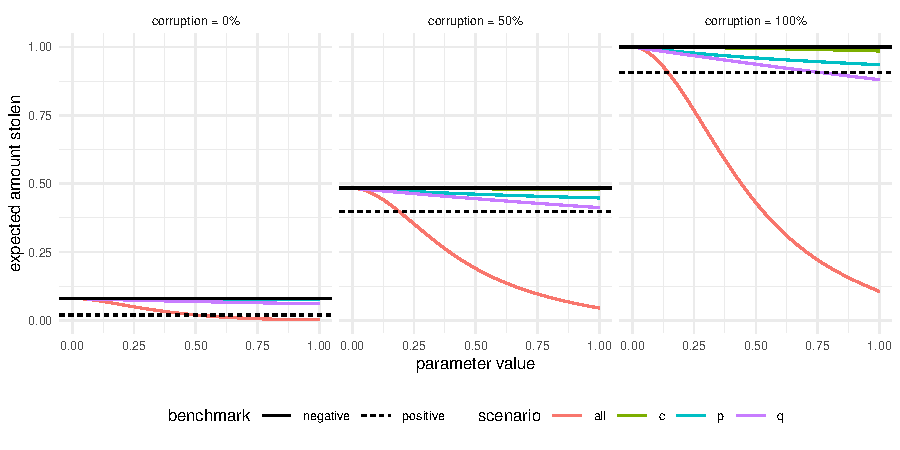
\includegraphics{chapters/chapter_2/figures/counterfactuals_effectiveness.pdf}
    \caption{{\bf Impact of increasing parameter values on total expected corruption.} When considering each component of the program in isolation, increasing the strength of monitoring associated with audits $q$ is the most effective approach. Program components display strong complementarities: increasing all parameters jointly is by far more effective than increasing any parameter in isolation.}
    \label{fig:counterfactuals2}
\end{figure}

Overall, our results paint a nuanced picture of the effect of the audits program on bureaucratic careers and corruption. Both structural and reduced-form results show that audits have caused small ex-post reductions in corruption. Furthermore, while bureaucrats stay in office much more than what is to be expected given their private/public-sector wage differential, it is unclear whether this owes to strong public-sector motivation, or pervasive rents from corruption. Finally, The program could be made more effective by making the monitoring component of audits more effective and, mostly, by leveraging strong complementarities among program components: a multi-pronged approach of making small improvements to the frequency, monitoring, and clean-up effects of audits is far more effective than making large improvements in a single component of the program. 

\section{Conclusion}
\label{sec:conclusion}

% Corruption is endemic across the developing world. Policies designed to reduce it have to carefully consider how they will affect the behavior of different types of public officials. We considered a program that has been shown to be effective at disciplining politicians, and considered its effect on bureaucrats. A first series of reduced-form analyses compared audited municipalities to municipalities that had not been audited yet, in order to investigate the short term effect of audits on careers. This analysis revealed that audits have no significant observable, ex-post effects on bureaucrats' careers: after an audit, bureaucrats do not get dismissed nor depart from the bureaucracy, suggesting that audits potentially have little effect on corruption. 

% This reduced-form approach, however, has a few shortcomings. Specifically, it is by design, unable to reveal potential unobservable ex-post effects on corruption (i.e. bureaucrats refraining from corruption without interrupting their career), nor potential disciplining effects. As such, this approach might have overlooked channels through which the program could be effective. 

% In response to these shortcomings, we devised a theoretical model that takes into account how the specifics of bureaucratic careers -- as opposed to politicians' -- feature in their decision to engage in corruption. Specifically, when deciding whether to engage in corruption, bureaucrats weigh their exit options against an extended career time-horizon. In this environment, audits may have a wide array of effects. Those range from disciplining effects, when audits induce strong sanctions, to ex-post effects, including temporary lapses in corruption, or waves of career interruptions, as those sanctions become less severe. In the limit, sanctions are not severe enough to induce any reduction in corruption. 

Corruption is endemic across the developing world. Policies designed to reduce it have to carefully consider how they will affect the behavior of different types of public officials. We considered a program that has been shown to be effective at disciplining politicians, and considered its effect on bureaucrats. We devised a theoretical model that takes into account how the specifics of bureaucratic careers -- as opposed to politicians' -- feature in their decision to engage in corruption. Specifically, when deciding whether to engage in corruption, bureaucrats weigh their exit options against an extended career time-horizon, leading to a wide range of potential ex-post, or disciplining effects. 

Taking the model to the data showed that audits have little ex-post effects, and that bureaucrats remain in office much more than what would be expected given their public/private-sector wage differential: bureaucrats receive a time- and large municipality-invariant payoff that amounts to 90\% of the median public-sector wage. We are, however, unable to tell whether this payoff stems from high public sector motivation or from pervasive rents from corruption. In other words, results suggest that the program either has a large disciplining effect or no effect at all. 

Our results have important implications for the design of effective anti-corruption policies. Investigating ways to make the program more effective, we found that the three components of the program; namely, the frequency of audits, the quality of monitoring, and the size of bureaucratic clean-ups show strong complementarities. Out of all three components, increasing the strength of the monitoring associated with audits is most effective at curbing corruption, as suggested by previous studies \citep{olken_monitoring_2007,bobonis2016,zamboni_audit_2018}. However, improving all three components jointly is far more effective than working in isolation: improving all components to 25\% is more effective than perfectly punishing corruption. This suggests that multi-pronged approaches aiming at reinforcing jointly all components of a policy are more effective than narrower, single-pronged approaches. 

Our paper proposes an alternative approach to policy evaluation, that usefully complements randomized controlled trials (RCTs), a practice that has become increasingly common in the development community \citep{deaton2010instruments}. Using structural estimation, our approach features a tight linkage between theory and empirics. The first benefit is breaking down a complex, nation-wide policy into simple constitutive components, and manipulating each of those separately. This allows us to assess the effectiveness of the program by comparing to a counterfactual in which it never took place -- which RCTs already do -- while also considering counterfactuals in which we manipulate each of its components individually or jointly. A second benefit is that we are able to identify, through theory, unobservable and long-term disciplining effects. In our particular setting, a reduced-form approach would have missed such long-term effects. These benefits, however, come at a cost: our estimation relies on stronger assumptions which RCTs, by design, do not, and we are unable to ascribe such long-term effects to large public sector motivation or pervasive rents from corruption. Nevertheless, designing similar policy evaluations using RCTs requires complex interventions that may not be feasible in practice. Overall, we advocate for complementary approaches to policy evaluation which leverage the comparative advantages of each. 

Finally, an important line of inquiry is to investigate the generalizability of our findings. While we provide a theoretical framework that could, \emph{a priori}, extend to any other audit program, several points may not generalize as easily. First, while a large number of countries introduce some randomness in their audits, full randomization is not a common feature, as countries tend to prioritize those places that are more likely to be corrupt. Our model could accommodate this by making the probability of an audit depend on the results of the previous audit. Second, our particular program showed little ex-post effect because audits fail to trigger large waves of dismissals or departures in corrupt municipalities. Investigating the reasons behind this in our context may help predict whether a similar policy will show comparable effects in other settings. We surmise that this owes to the facts that (1) audits occur infrequently because they are costly, and (2) that unionization introduces additional frictions that shelter corrupt bureaucrats from punishment. Lastly, we showed that the program exhibits strong complementarities. Further research could explore whether similar complementarities apply in other settings. 

% \newpage

% \bibliography{dissertation_dedup}

\newpage
\section{Appendix}

\appendixpage

% \startcontents[sections]
% \printcontents[sections]{l}{1}{\setcounter{tocdepth}{2}}

\subsection{Proofs}
\label{app:proofs}

In this section, we denote by $v_\pi(s) = \mathbb{E}_\pi \left[ (1-\de) \sum_{t = 0}^\infty \delta^t u(\pi(s_t), s_t) | s_0 = s \right]$ the continuation value implied by a strategy in state $s$. We denote by $\pi_0, \pi_1, \pi_2$  the policies that consist in playing 0, 1, 2 respectively in both states $A$ and $N$. Note that $v_{\pi_0} = w$ and $v_{\pi_2} = \wb$. For concision, we also define $\pb \equiv pq$. Since the action and state spaces are both small, we check for optimality by comparing the value functions of all possible policies. 

\begin{proof}[Proof of proposition \ref{prop:eq0}]
    Note that 
    $$
    v_{\pi^*}(N) = v_{\pi^*}(A) = (1-\de) (w+b) + \de [(1-\pb) v_{\pi^*}(N) + \pb \wb]
    $$
    Solving for $v_{\pi^*}(N)$, we get
    $$
    v_{\pi^*}(N) = \frac{(1-\de)(w+b)+\de \pb \wb}{1 - (1-\pb)\de}
    $$
    Note that $v_{\pi^*}(N) > \wb \iff w + b > \wb$, which is true by assumption. So $\pi^*$ is always preferred to $\pi_2$. Also note that $v_{\pi^*}(N) > w \iff b (1-\de) + \pb (\wb - w) \de > 0$. As such, if $\wb > w$, then $\pi^*$ is always preferred to $\pi_0$. If $\wb < w$,  $\pi^*$  is preferred to $\pi_0$ iff $b \geq \frac{\pb (w - \wb) \de}{1-\de} \equiv b_0 > 0$.
\end{proof}

\begin{proof}[Proof of proposition \ref{prop:eqK}]
    Note that 
    $$
    v_{\pi_1}(N) = v_{\pi_1}(A) = (1-\de) (w+b) + \de [(1-\pb) v_{\pi_1}(N) + \pb (\wb - (1-\de) k)]
    $$
    Solving for $v_{\pi_1}(N)$, we get
    $$
    v_{\pi_1}(N) = \frac{(1-\de)(w+b-\de\pb k)+\de\pb \wb}{1-\de(1-\pb)}
    $$
    If $w < \wb$ (i.e. if equation \ref{eq:wwb} holds), then $\pi_2$ is preferred to $\pi_0$. We have that 
    $$
    v_{\pi_1}(N) \geq v_{\pi_2}(N) \iff k \leq \frac{w+b-\wb}{\pb\de} \equiv k_0
    $$
    Yet, $k_0 \leq \wb \iff \wb \geq \frac{w+b}{1+\de\pb} > w+b$, which is impossible. As such $v_{\pi_1}(N) \geq v_{\pi_2}(N)$ for any $k \in [0,\wb]$, so $\pi_1$ is optimal. 

    Suppose now that $\wb < w$ (i.e. suppose that equation \ref{eq:wbw} holds). In this case, $\pi_0$ is preferred to $\pi_2$. We have that 
    $$
    v_{\pi_1}(N) \geq v_{\pi_0}(N) \iff k \leq \frac{(1-\de)b-\pb\de(w-\wb)}{(1-\de)\pb\de} \equiv k_0
    $$
    We have that $k_0 \geq 0 \iff b \geq \frac{\pb\de(w-\wb)}{1-\de} \equiv b_0$. We have that $k_0 \leq \wb \iff b \leq \frac{\pb\de(w-\wb\de)}{1-\de} \equiv b_1 > b_0$. 
\end{proof}

\begin{proof}[Proof of proposition \ref{prop:eqC}]
    Note first that if a policy $\pi^*$ such that $\pi^*(A) = 1$ is optimal, then it must be that $\pi^* = \pi_1$. Indeed, the continuation values of policy $\pi_1$ satisfy the following: 
    \begin{align*}
        v_{\pi_1}(N) =& (1-\de) (w+b) + \de [(1-p) v_{\pi_1}(N) + p(1-q) v_{\pi_1}(A) + \pb \wb] \\ 
        v_{\pi_1}(A) =& (1-\de) (w+b-c) + \de [(1-p) v_{\pi_1}(N) + p(1-q) v_{\pi_1}(A) + \pb \wb]
    \end{align*} 
    Since $c > 0$, we have that $v_{\pi^*}(A) = v_{\pi_1}(A) < v_{\pi_1}(N)$. Furthermore, since $\pi^*(A) = 1$ is optimal, then it must be that $v_{\pi^*}(A) \geq \wb$. As such, it cannot be that $\pi^*(N) = 2$, because this would imply that $v_{\pi^*}(N) = \wb < v_{\pi_1}(N)$. Suppose now that $\pi^*(N) = 0$. Then $v_{\pi^*}(N) = (1-\de) w + \de [(1-p) v_{\pi_1}(N) + p v_{\pi_1}(A)]$. Yet, if $\pi^*(A) = 1$ is optimal, then such policy is preferred to a policy $\pi'$ such that $\pi'(A) = 0$ and $\pi'(N) = 1$. As such, we have $v_(\pi^*)(A) \geq v_{\pi'}(A) = v_{\pi^*}(N)$. Yet, we have $v_{\pi_1}(N) > v_{\pi^*}(A) \geq v_{pi^*}(N)$, a contradiction. 

    Note furthermore that since $w > \wb$ or $\wb > w$, a policy such that $\pi(N), \pi(A) \in \{0,2\}$ and $\pi(N) \neq \pi(A)$ is suboptimal, as either $v_{\pi_0}(s) > v_\pi(s)$ or $v_{\pi_2}(s) > v_\pi(s)$ for $s \in \{A, N\}$. 

    As such, the remaining policies are $\pi_0$, $\pi_1$, $\pi_2$, and policies $\pi_{10}$ and $\pi_{12}$ which correspond to $\pi(N) = 1$, and $\pi(A) = 0, 2$ respectively.
    
    Solving for $v_{\pi_1}(N), v_{\pi_1}(A)$, we get
    \begin{align*}
        v_{\pi_1}(N) =& \frac{(1-\de)[b+w-\de p(1-q)c]+\de\pb\wb}{1 - \de(1-\pb)} \\ 
        v_{\pi_1}(A) =& \frac{(1-\de)[b+w-(1-\de(1-p))c]+\de\pb\wb}{1 - \de(1-\pb)}
    \end{align*}

    Continuation values for $\pi_{10}$ satisfy
    \begin{align*}
        v_{\pi_{10}}(N) =& (1-\de) (w+b) + \de [(1-p) v_{\pi_{10}}(N) + p (1-q) v_{\pi_{10}}(A) + \pb \wb] \\ 
        v_{\pi_{10}}(A) =& (1-\de) w + \de [(1-p) v_{\pi_{10}}(N) + p v_{\pi_{10}}(A)]
    \end{align*}
    Solving for $v_{\pi_{10}}(N), v_{\pi_{10}}(A)$, we get
    \begin{align*}
        v_{\pi_{10}}(N) =& \frac{(1-\de)[(1-p\de)b+(1-\pb\de)w]+\pb\de(1-p\de)\wb}{1-\de[1-(1-p)\pb\de]}\\
        v_{\pi_{10}}(A) =& \frac{(1-\de)[w+(1-p)\de b]+\de^2\pb(1-p)\wb}{1-\de[1-(1-p)\pb\de]}&
    \end{align*}

    Finally, continuation values for $\pi_{12}$ satisfy
    \begin{align*}
        v_{\pi_{12}}(N) =& (1-\de) (w+b) + \de [(1-p) v_{\pi_{12}}(N) + p\wb] \\ 
        v_{\pi_{12}}(A) =& \wb
    \end{align*}
    Solving for $v_{\pi_{12}}(N)$, we get
    $$
    v_{\pi_{12}}(N) = \frac{(w+b)(1-\de)+p\de\wb}{1-(1-p)\de}
    $$

    Suppose first that $w < \wb$ (case \ref{eq:wwb}). Note that in this case, $v_{\pi_2}(s) = \wb > v_{\pi_1}(s) = w$ for any $s \in \{A,N\}$. Also note that since $w+b > \wb$, we have that $v_{12}(N) > v_{\pi_2}(N)$. As such, three policies remain: $\pi_{12}, \pi_{10}$, and $\pi_1$. 

    We have $v_{\pi_1}(N) \geq v_{\pi_{12}}(N) \iff c \leq \frac{w+b-\wb}{1-(1-p)\de} \equiv c_1$, and $c_1 \leq b \iff b \leq \frac{\wb-w}{\de(1-p)} \equiv b_0$. 

    We have $v_{\pi_1}(N) \geq v_{\pi_{10}}(N) \iff c \leq \frac{(1-\de)b+\pb\de(\wb-w)}{1-\de[1-(1-p)\pb\de]} \equiv c_2$, and $c_2 \leq b \iff b \geq b_0$. 

    So $v_{\pi_1}(N) = \max_{\pi} v(N) \iff c \leq \overline{c} \equiv \max\{c_1, c_2\}$. Furthermore, $v_{\pi_{12}}(N) = \max_{\pi} v(N) \iff c \leq \overline{c}$ and $b \leq b_0$. Conversely, $v_{\pi_{10}}(N) = \max_{\pi} v(N) \iff c \leq \overline{c}$ and $b \geq b_0$. We show similarly that this holds true for state $A$. 

    Suppose now that $w > \wb$ (case \ref{eq:wbw}). Note that in this case, $v_{\pi_2}(s) = \wb < v_{\pi_1}(s) = w$ for any $s \in \{A,N\}$. Also note that since $w > \wb$, we have that $v_{\pi_{10}}(s) > v_{\pi_{12}(s)}$ for any $s \in \{A,N\}$. As such, three policies remain: $\pi_0, \pi_{10}, \pi_1$. 

    We have $v_{\pi_1}(N) \geq v_{\pi_{10}}(N) \iff w \leq \frac{b(1-\de)+\pb\de\wb-c[1-\de(1-(1-p)\pb\de)]}{\pb\de}  \equiv w_2$. Also note that $w_2 \geq \wb \iff b \geq c \frac{1-\de[1-(1-p)\pb\de]}{1-\de} \equiv b_2$. 

    Furthermore, we have $v_{\pi_{10}}(N) \geq v_{\pi_0}(N) \iff w \leq \frac{b(1-\de)+\pb\de\wb}{\pb\de}\equiv w_1$. Also note that $w_1 \geq \wb \iff b \geq 0$, and that $w_1 \geq w_2$.  

\end{proof}

\subsection{Additional descriptive statistics}
\label{app:descriptives}

\subsection{Measuring corruption}
\label{app:fault}

\subsubsection*{Sampling from audit reports} 

We draw a random sample of 30 reports to verify how infractions were classified into two categories: \textit{grave}, and \textit{media}. \textit{Falhas graves} are really the ones we focus on as evidence of corruption. In this category, auditors report practices that are clearly associated with corruption: collusion between companies and government, over invoicing of budgets, withholding of salaries or spending on staff members who are not allowed to be hired by the program.

In the category \textit{falhas medias}, we have minor infractions that are not necessarily evidence of corruption, but procedural deficiencies. For instance, we have  some municipalities that fail to respect a regular meeting of the health board, or that fail to provide enough books in school. We do not believe that constitutes enough evidence of corruption, since this seems to be rather weaknesses in administrative procedure that are meant to be identified by these audits.

\begin{itemize}
    \item \textbf{Falha m\'{e}dia:} Minor irregularities in the execution of programs. Mostly attributed to deficiencies in administrative procedure, rather than clear examples of corrupt behavior. Examples: 1) there is not a schedule for school bus maintenance, 2) not enough books in school; 3) poor infrastructure for healthcare facilities; 4) mismatch between registered beneficiaries and eligible families for Bolsa Família; 4) no formal procedure for legal actions in the health council.
    \item \textbf{Falhas graves:} The relevant category for corruption. In this category, we find evidence of over budgeting, illicit subcontracting practices, ghost employees, payment for services never provided. Examples: 1) requirements in audit that favor a particular company; 2) overspending of items in the budget, without justification; 3) charge for conditional cash transfers; 4) public servants receive Bolsa Família, when clearly above the income threshold.
\end{itemize}

\subsubsection*{Constructing measures of corruption}

In this section, we report the correlation among all measures of corruption, and show evidence for a time trend. The stringency of auditing criteria has varied over time, with audits picking up increasingly many intermediate faults until lottery 25, and fewer after lottery 35. We remove this time trend by de-meaning irregularity counts by lottery, and validate our four measures by verifying that they reproduce the main finding of \citet{avis_government_2018}; namely, that municipalities that have been audited twice show less corruption on their second audit. In the analysis, we group municipalities into terciles, creating equal-sized groups of low-, moderate- and high-corruption municipalities. 

\begin{figure}[H]
    \centering
    \begin{subfigure}[b]{0.49\textwidth}
        \centering
        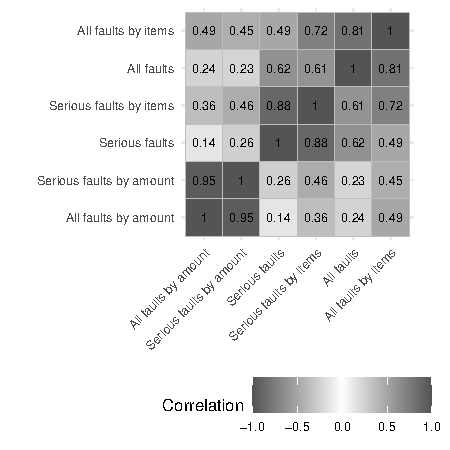
\includegraphics{chapters/chapter_2/figures/corruptionCorrelation}
        \caption{Correlation among corruption metrics}
        \label{fig:corruptionCorrelation}
    \end{subfigure}
    \begin{subfigure}[b]{0.49\textwidth}
         \centering
         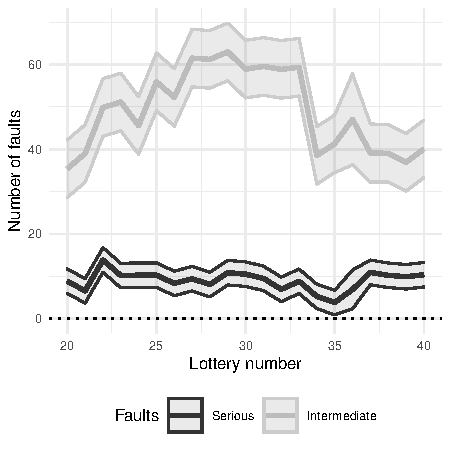
\includegraphics{chapters/chapter_2/figures/corruptionOverTime}
         \caption{Mean number of faults over time}
         \label{fig:corruptionOverTime}
     \end{subfigure}
    \caption{{\bf Constructing indicators of corruption.} Left: While many corruption metrics are highly correlated, least correlation ($< .5$) is found between the metrics that are normalized by amount audited and the other metrics. Right: Audits become more stringent from lottery 20 to 27, then less stringent from lottery 32 onwards, as evidenced by the mean number of intermediate faults picked up by an audit (shaded areas are 95 percent heteroskedastic-robust confidence intervals).}
    \label{fig:auditsOverTime}
\end{figure}

\begin{figure}[H]
    \centering
    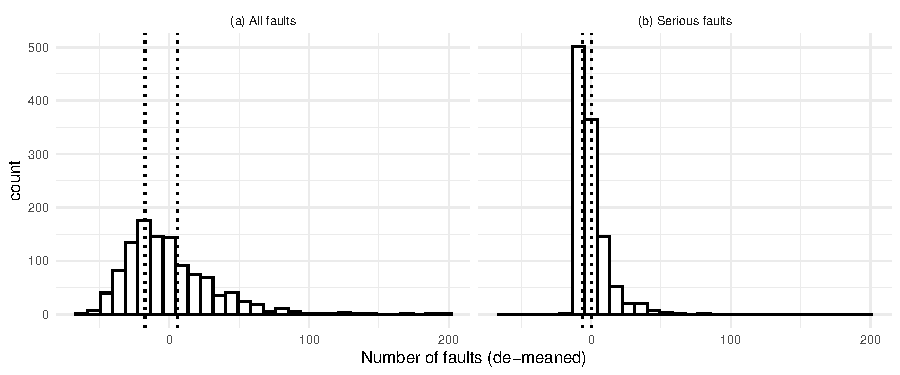
\includegraphics{chapters/chapter_2/figures/distribNIrregularities}
    \caption{{\bf Distribution of number of irregularities.} Vertical bars indicate the first and second tercile of each distribution. Most municipalities show little corruption.}
    \label{fig:distribIrregularities}
\end{figure}

\begin{landscape}
    \subsubsection*{Validation: Replication of \citet{avis_government_2018}}
    \label{app:replication}

    \begin{table}[H]
        \centering
        \footnotesize
        
% Table created by stargazer v.5.2.2 by Marek Hlavac, Harvard University. E-mail: hlavac at fas.harvard.edu
% Date and time: Tue, Jun 02, 2020 - 01:02:39 PM
\begingroup 
\small 
\begin{tabular}{@{\extracolsep{5pt}}lcccccccc} 
\\[-1.8ex]\hline 
\hline \\[-1.8ex] 
 & \multicolumn{8}{c}{\textit{Dependent variable:}} \\ 
\cline{2-9} 
\\[-1.8ex] & \multicolumn{2}{c}{All} & \multicolumn{2}{c}{Serious} & \multicolumn{2}{c}{All per Amount} & \multicolumn{2}{c}{Serious per Amount} \\ 
\\[-1.8ex] & (1) & (2) & (3) & (4) & (5) & (6) & (7) & (8)\\ 
\hline \\[-1.8ex] 
 treat & $-$0.035$^{*}$ & $-$0.041$^{**}$ & $-$0.0003 & $-$0.017 & $-$0.150$^{***}$ & $-$0.055 & $-$0.093$^{*}$ & $-$0.059 \\ 
  & (0.019) & (0.019) & (0.057) & (0.057) & (0.056) & (0.036) & (0.049) & (0.046) \\ 
 \hline \\[-1.8ex] 
Controls & \_ & \checkmark & \_ & \checkmark & \_ & \checkmark & \_ & \checkmark \\ 
\citet{avis_government_2018} & \checkmark & \checkmark & \_ & \_ & \_ & \_ & \_ & \_ \\ 
Observations & 1,095 & 1,095 & 1,095 & 1,095 & 1,095 & 1,095 & 1,095 & 1,095 \\ 
R$^{2}$ & 0.792 & 0.796 & 0.509 & 0.516 & 0.386 & 0.742 & 0.203 & 0.303 \\ 
\hline 
\hline \\[-1.8ex] 
\textit{Note:}  & \multicolumn{8}{r}{$^{*}$p$<$0.1; $^{**}$p$<$0.05; $^{***}$p$<$0.01} \\ 
\end{tabular} 
\endgroup 

        \caption{{\bf Replication of \citet{avis_government_2018}.} All models include lottery and state fixed effects and use robust standard errors. Models (1) and (2) replicate the specification in \citet{avis_government_2018} on an extended time period. Models 1-4 control for the log number of audited items. Models 4-8 do not. Results are largely robust to alternative specifications of the dependent variable.}
        \label{tbl:replication}
    \end{table}    
\end{landscape}

\subsection{Management index} \label{app:mgmt}

\subsubsection*{Details about construction}

In this section, we outline in depth how the management index is constructed. Information is gathered from the \textit{Pesquisa de Informações Básicas Municipais} (Munic), an annual census conducted by the Institute of Brazilian Geography and Statistics (IBGE). The questionnaire is self-reported by municipalities, gathering information on a set of administrative practices, indicating the presence or not of a certain institutional feature or practice.

To construct the index $m_{jt}$ for municipality $j$ at year $t$, we use a similar approach to \cite{Bloom2007} deploy to compare management practices among firms. We construct three dimensions of "good" management that can potentially reduce corruption. Table \ref{tbl:mgmtIndex} provides a random sample of 5 practices per dimension to illustrate the types of management practices used to calculate the management index.

\begin{table}[H]
	\begin{table}[H]
\centering
\begin{tabular}{rl}
\toprule
Year & Practice\\
\midrule
\addlinespace[0.3em]
\multicolumn{2}{l}{\textbf{Accountability}}\\
\hspace{1em}2005 & Culture Council\\
\hspace{1em}2009 & Urban Policy Council\\
\hspace{1em}2012 & Council for Physical Disability Rights\\
\hspace{1em}2013 & Health Council\\
\hspace{1em}2013 & Environmental Council\\
\addlinespace[0.3em]
\multicolumn{2}{l}{\textbf{Accounting}}\\
\hspace{1em}2004 & Property Registration\\
\hspace{1em}2009 & Digital Property Registration\\
\hspace{1em}2011 & Families in Housing Programs Registration\\
\hspace{1em}2013 & Housings Programs Registration\\
\hspace{1em}2013 & Population at Risk Registration\\
\addlinespace[0.3em]
\multicolumn{2}{l}{\textbf{Planning}}\\
\hspace{1em}2008 & Transportation Planning\\
\hspace{1em}2009 & City Planning\\
\hspace{1em}2012 & Transportation Planning\\
\hspace{1em}2012 & Food Safety and Nutrition Planning\\
\hspace{1em}2014 & Food Safety and Nutrition Planning\\
\bottomrule
\end{tabular}
\end{table}
	\caption{Random sample of administrative practices, broken down by each respective dimension. Note that the questions can vary according to the year in which the questionnaire is administered.}
	\label{tbl:mgmtIndex}
\end{table}

Within each of these dimensions, we count the number of practices $n_{jt}$  in municipality $j$ at time $t$. Note that the index is time variant: the number of practices vary from year to year, due to modifications in the structure of the questionnaire. We then take an arithmetic mean across the three $k$ dimensions.

$$m_{jt} = \frac{1}{3} \sum_{k = 1}^{3} \frac{n_{kjt}}{n_{kt}}$$

\subsubsection*{Validation}

\begin{figure}[H]
    \centering
    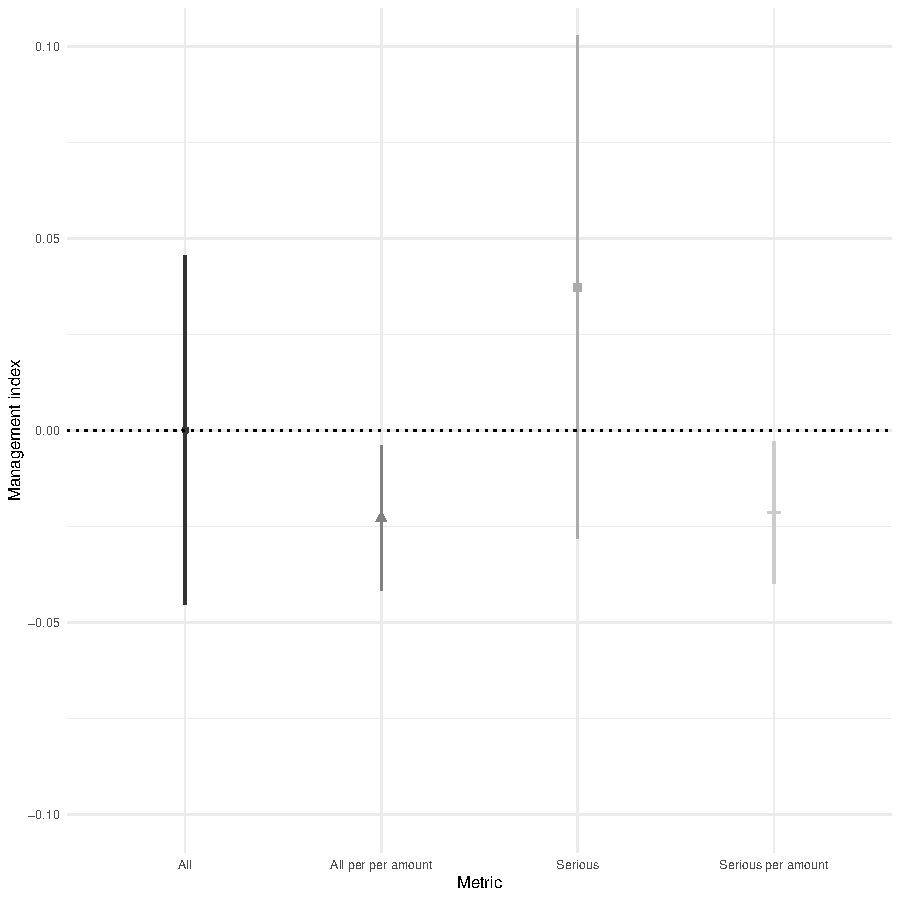
\includegraphics{chapters/chapter_2/figures/managementCorruption.pdf}
    \caption{{\bf Correlation management index - corruption.} We find partial support for the hypothesis that more corrupt municipalities have poorer management. This figure reports the coefficient associated with regressing the management index in municipality $j$ as measured by the Munic survey conducted in period $t$ on corruption as measured by audit conducted in period $t+1$. State and year fixed effects, controlling for Gini coefficient, illiteracy rate, population size and total number of items audited. Standard errors are clustered at the municipal level.}
    \label{fig:correlationMgmtCorruption}
\end{figure}

\subsection{Additional descriptive statistics}
\label{app:additional_descriptives}

\begin{figure}[H]
    \centering
    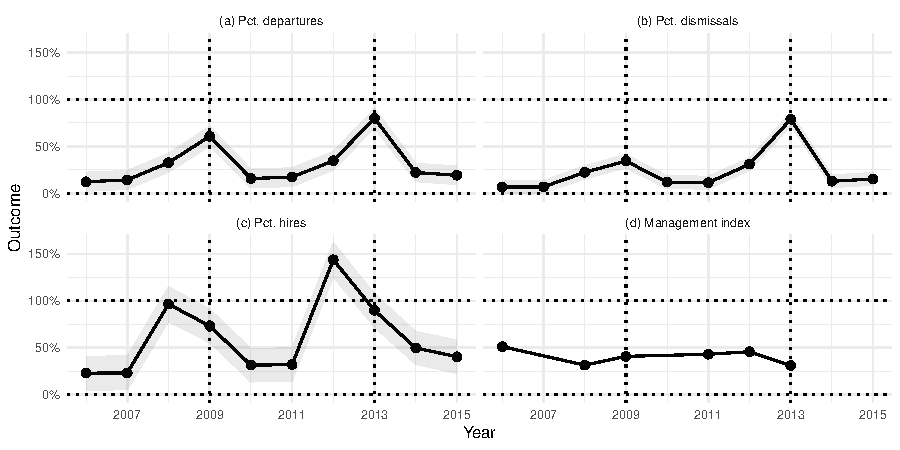
\includegraphics{chapters/chapter_2/figures/dependentVariables}
    \caption{{\bf Dependent variables over time.} Vertical bars denote election years. Shaded areas are heteroskedastic-robust 95 percent confidence intervals. There is seasonality in staff rotation around election years (panels a, b, c). On average, management practices remain constant over time.}
    \label{fig:dvs}
\end{figure}

\section{Robustness checks}
\label{app:robustness}

\subsection{Other categories of bureaucrats}
\label{app:otherBureaucratsRobustness}

\begin{figure}[H]
    \centering
    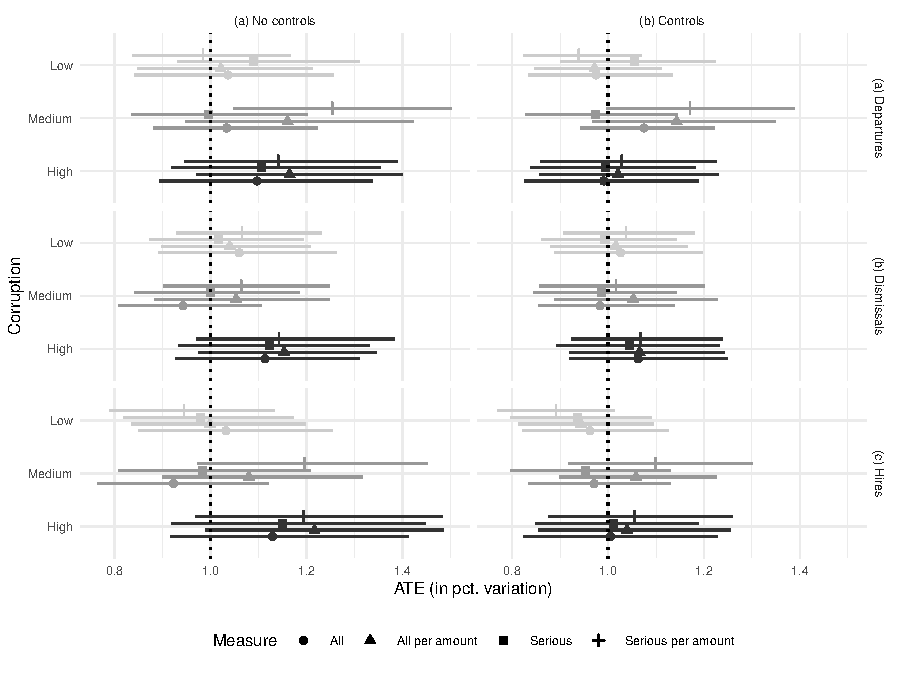
\includegraphics{chapters/chapter_2/figures/pl_bureaucrat_low.pdf}
    \caption{{\bf Low bureaucrats.} This figure reproduces Figure \ref{fig:mainPl} in the main text but considers low bureaucrats instead of high bureaucrats.}
    \label{fig:plLowBureaucrats}
\end{figure}

\begin{figure}[H]
    \centering
    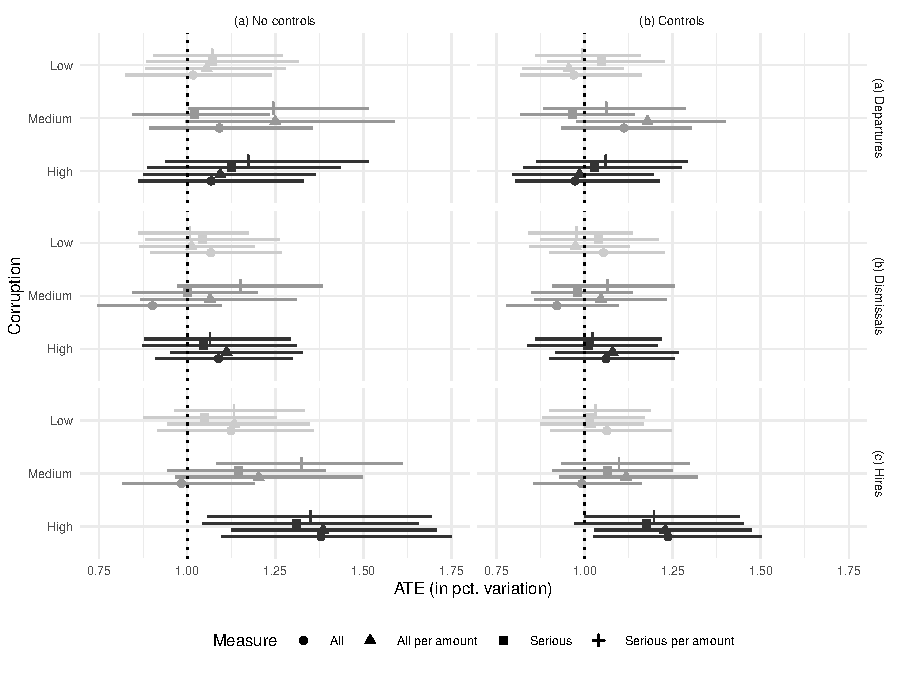
\includegraphics{chapters/chapter_2/figures/pl_frontline_high.pdf}
    \caption{{\bf High Frontline.} This figure reproduces Figure \ref{fig:mainPl} in the main text but considers high frontline providers instead of high bureaucrats.}
    \label{fig:plHighFrontline}
\end{figure}

\begin{figure}[H]
    \centering
    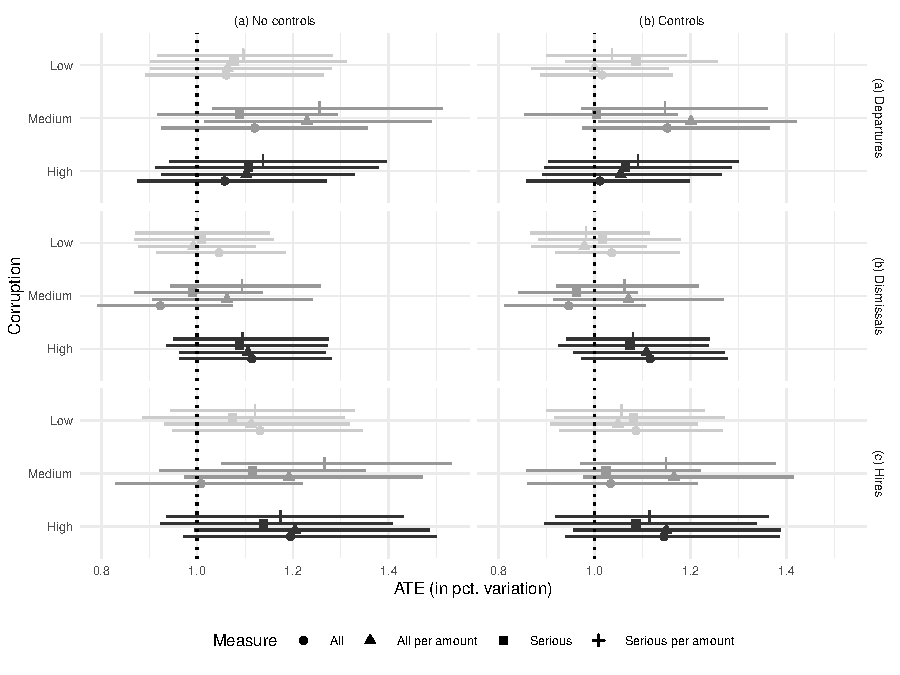
\includegraphics{chapters/chapter_2/figures/pl_frontline_low.pdf}
    \caption{{\bf Low Frontline.} This figure reproduces Figure \ref{fig:mainPl} in the main text but considers high frontline providers instead of high bureaucrats.}
    \label{fig:plLowFrontline}
\end{figure}

\subsection{Subset of municipal secretaries}
\label{app:secretariesRobustness}

\begin{figure}[H]
    \centering
    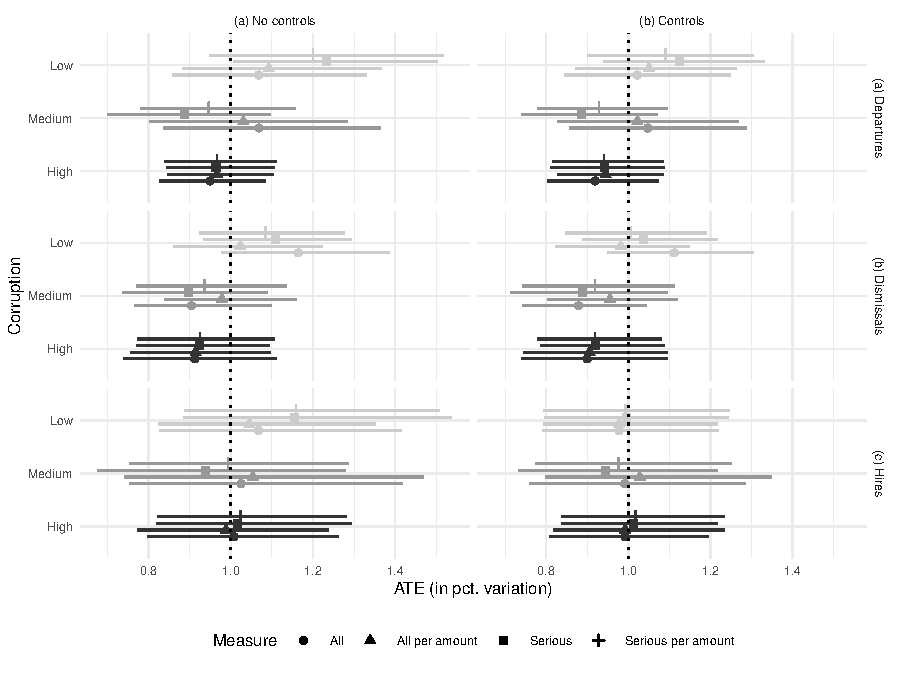
\includegraphics{chapters/chapter_2/figures/plSubset}
    \caption{{\bf Subset of municipal secretaries.} This figure reproduces Figure \ref{fig:mainPl} in the main text but restricts the sample to the highest-ranking bureaucrats, namely municipal secretaries.}
    \label{fig:plSubset}
\end{figure}

This robustness check focuses on the highest-ranking bureaucrats; namely, the set of municipal secretaries, who oversee municipal departments. Indeed, it might be the case that effects on personnel only affect those highest ranking employees. We find similar results. Unfortunately, this category is poorly identified by the standard classification of occupations (CBO), leaving us with municipalities that supposedly have no secretaries. We drop those from the sample. 

\subsection{Subset by Tenure}
\label{app:tenuredRobustness}

This robustness check verifies whether there are heterogeneities according to the type of contract that the high-level bureaucrat holds: tenured or untenured. We find similar results to our original findings, with no evidence of hetereogeneity in outcomes.

\begin{figure}[H]
    \centering
    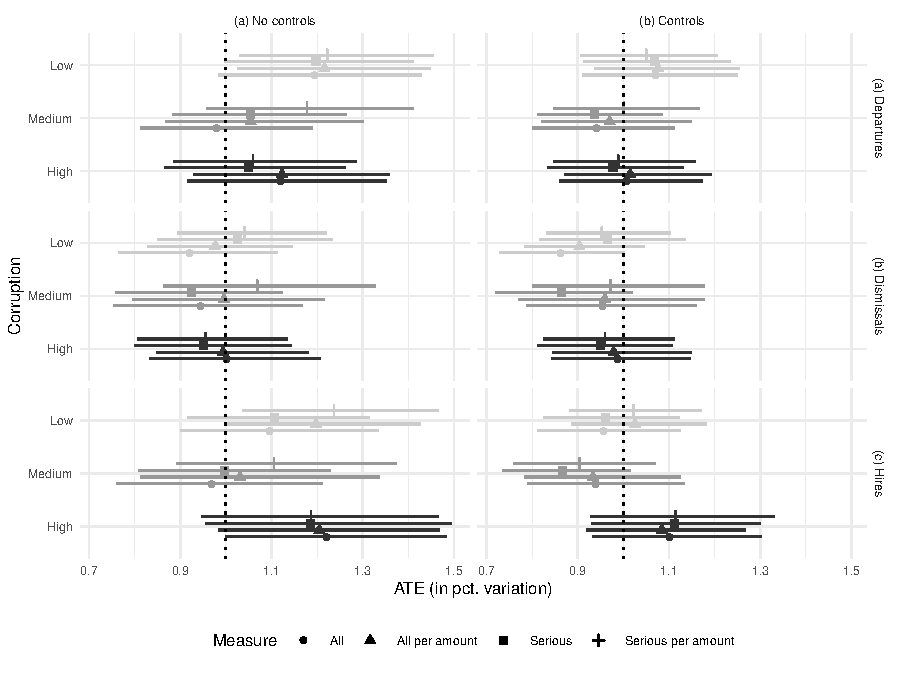
\includegraphics{chapters/chapter_2/figures/plSubsetTenured}
    \caption{{\bf Subset of tenured bureaucrats.} This figure reproduces Figure \ref{fig:mainPl} in the main text but splits the sample of highest-ranking bureaucrats into tenured bureaucrats.}
    \label{fig:plSubsetTenured}
\end{figure}

\begin{figure}[H]
    \centering
    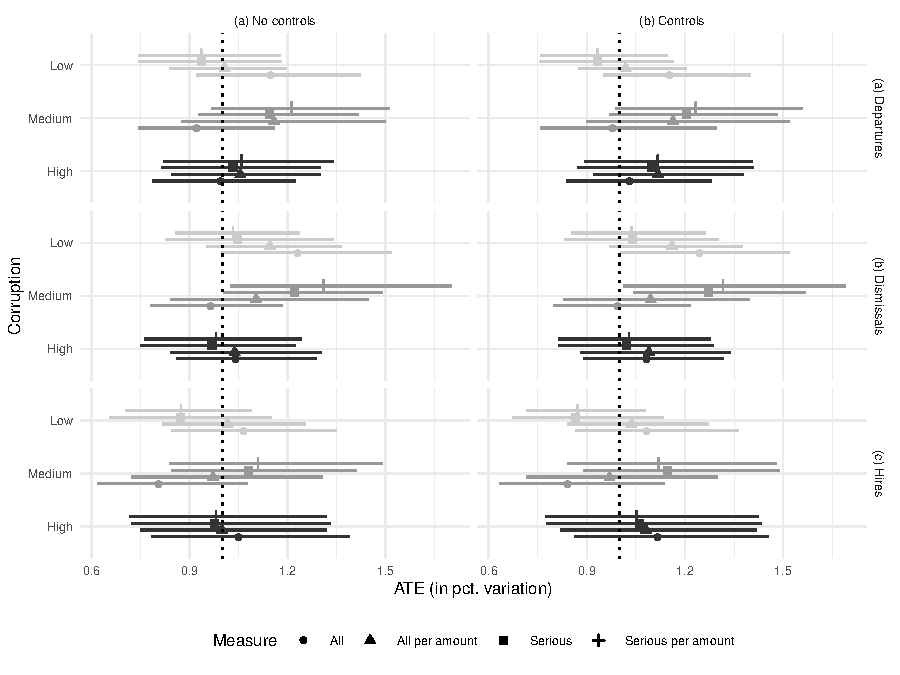
\includegraphics{chapters/chapter_2/figures/plSubsetUntenured}
    \caption{{\bf Subset of untenured bureaucrats.} This figure reproduces Figure \ref{fig:mainPl} in the main text but splits the sample of highest-ranking bureaucrats into untenured bureaucrats.}
    \label{fig:plSubsetUntenured}
\end{figure}

\subsection{Hiring Practices}
\label{app:hiring}
\begin{figure}[H]
    \centering
    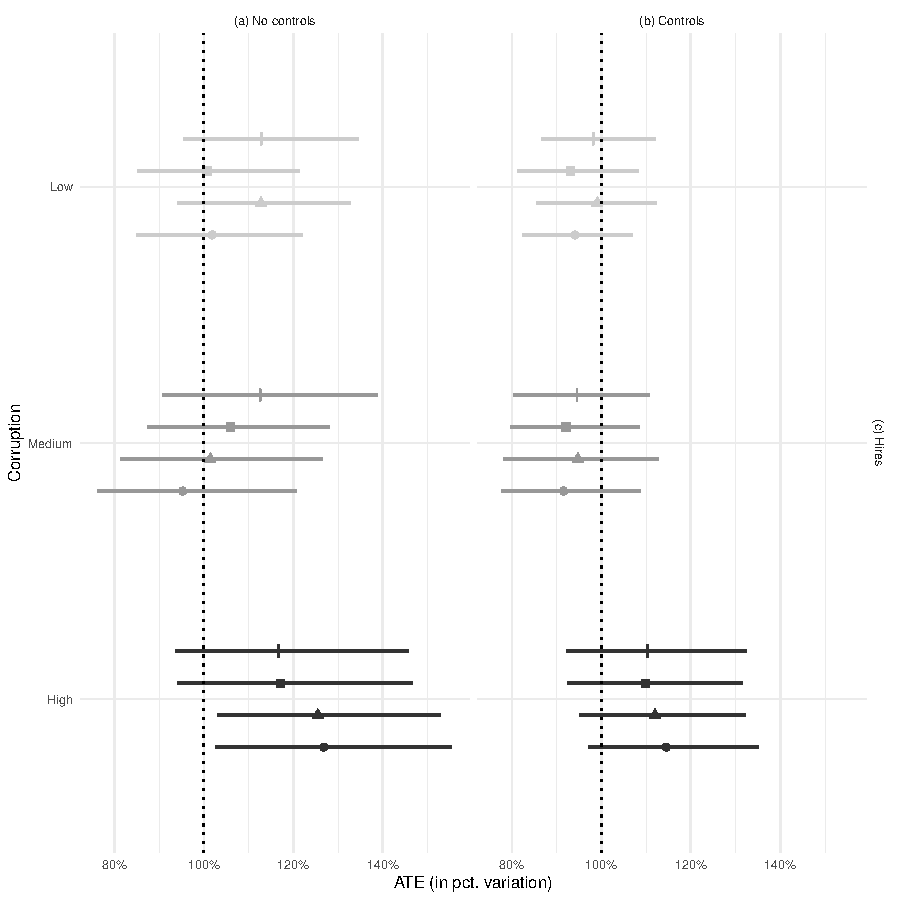
\includegraphics{chapters/chapter_2/figures/mainPlHires.pdf}
    \caption{{\bf Low bureaucrats.} This figure reproduces Figure \ref{fig:mainPl} in the main text but considers only hires.}
    \label{fig:plHires}
\end{figure}

\begin{figure}[H]
    \centering
    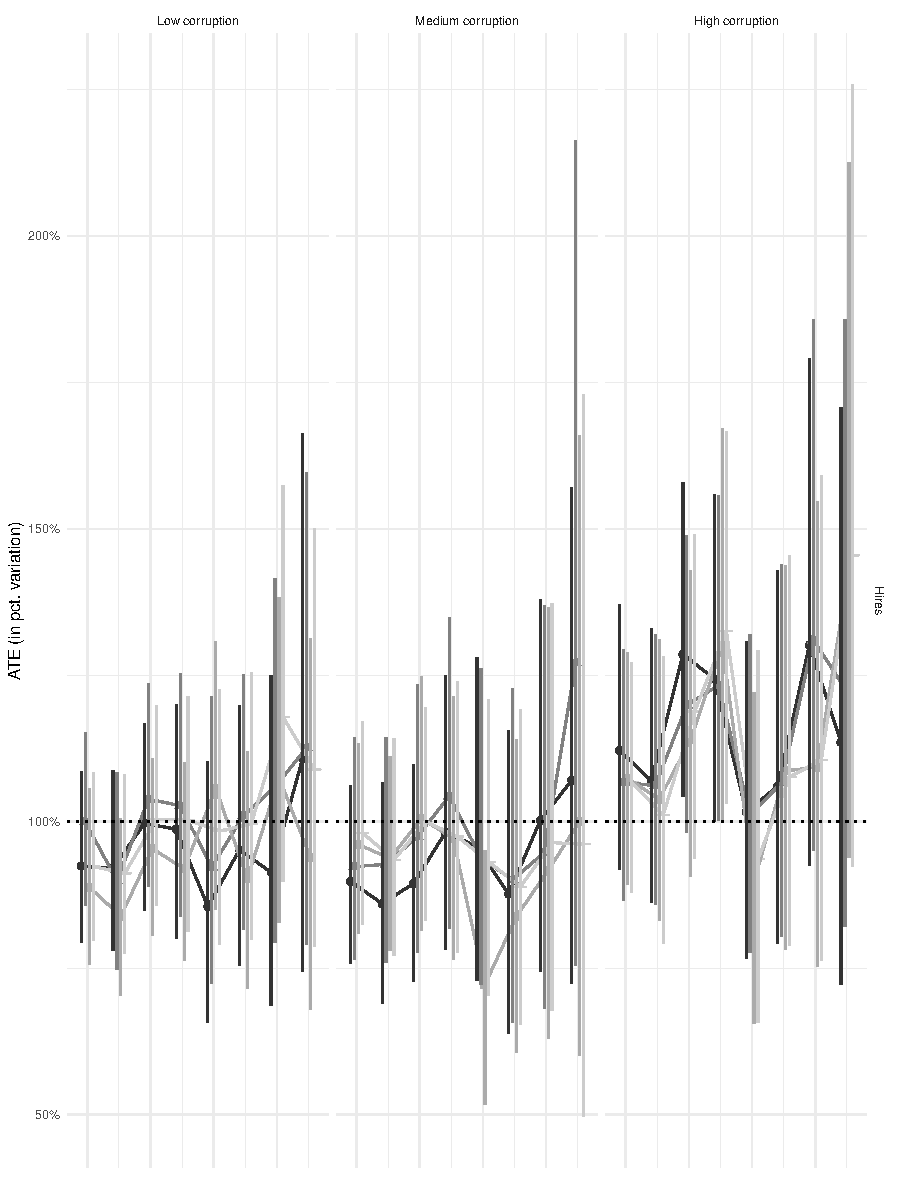
\includegraphics{chapters/chapter_2/figures/AMEoverTimeHires.pdf}
    \caption{{\bf High Frontline.} This figure reproduces Figure \ref{fig:AMEoverTime} in the main text but considers only hires.}
    \label{fig:AMEoverTimeHires}
\end{figure}

\subsection{Balance tests}
\label{app:balanceRobustness}

We verify audits' randomization procedure by comparing the set of municipalities that were audited early to those that were audited late, defining early and late as, respectively, before and after the median audit. 

% fix the sample size and remove DV's
% keep from number of bureaucrats (caption with 2006)
\begin{table}[H]
    
\begin{tabular}{llll}
\toprule
Variable & Early audit & Late audit & Diff in means (p-value)\\
\midrule
No. of bureaucrats (2006) & 97.214 & 64.879 & 32.335 (0.118)\\
Municipal population (logged) & 9.435 & 9.312 & 0.123 (0.057)*\\
Gini coefficient & 0.226 & 0.221 & 0.005 (0.469)\\
Illiteracy rate & 0.558 & 0.561 & -0.004 (0.385)\\
Median municipal wage & 190.73 & 189.245 & 1.484 (0.816)\\
\addlinespace
Urbanization & 0.579 & 0.58 & -0.002 (0.907)\\
Sample size & 5759 & 4397 & \\
\bottomrule
\end{tabular}
    \caption{\textbf{Covariate balance tests.} We check whether there are differences in the sample of municipalities audited early in the program (2006-9) with the later half in our sample (2009-2015). We regress each of our control variables against a dummy indicating whether the municipality was audited early, reporting the difference in means which corresponds to that coefficient. Standard errors are clustered at the municipal level. We find that none of the differences are statistically significant except for the logged municipal population, which may reflect later changes to the program which shifted priority to smaller municipalities.}
    \label{tbl:balance}
\end{table}

\subsection{Dependent variable as percentages}
\label{app:percentageRobustness}

This robustness check changes the dependent variable. Instead of using log counts, we follow \citet{poulsen2019corruption} and use the percentage of departures, dismissals, and hires. With $n_e$, $n_h$, $n_d$, $n_f$ the numbers of employees, hires, departures, and dismissals respectively, we compute:

\begin{align*}
    \text{pct. hire} &= \frac{n_h}{n_e - n_d - n_f}, \\ 
    \text{pct. departure} &= \frac{n_d}{n_e - n_h}, \\
    \text{pct. dismissal} &= \frac{n_f}{n_e - n_h}. 
\end{align*}

\begin{figure}[H]
    \centering
    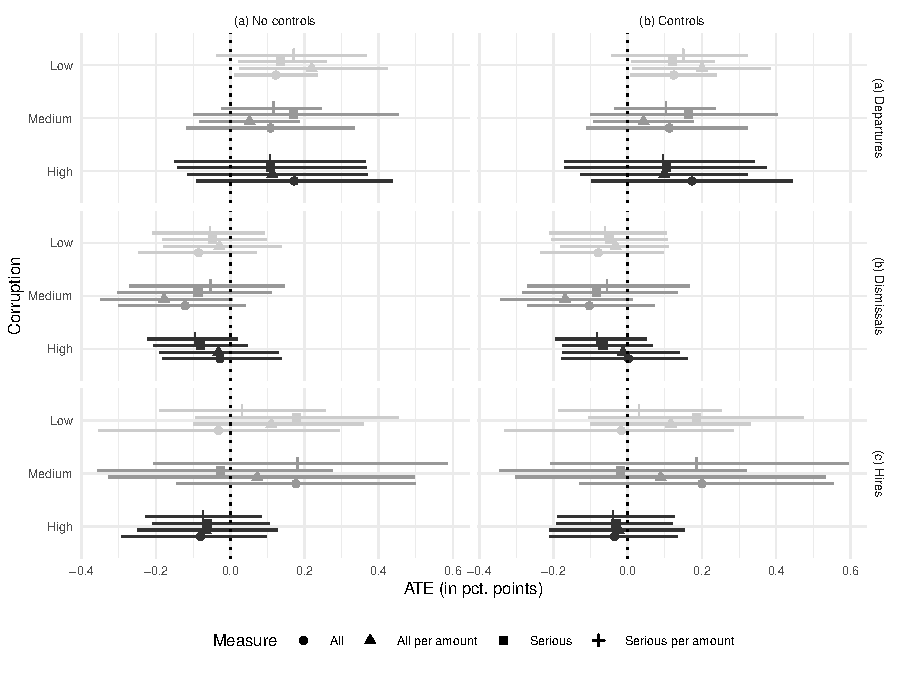
\includegraphics{chapters/chapter_2/figures/plDv}
    \caption{{\bf Dependent variable specified as percentages.} This figure reproduces Figure \ref{fig:mainPl} in the main text but specifies the dependent variables as percentages instead of log-counts. Findings are robust to this alternative specification of the dependent variable.}
    \label{fig:plDv}
\end{figure}

\subsection{Findings on management}
\label{app:managementRobustness}

In this section, we reproduce the bottom panel of Figure \ref{fig:mainPl} but vary the number of items used to construct the management index. The measure used in the main text uses all survey items that were asked in at least one wave. Here, we make this index increasingly restrictive by using only the items that were asked in at least two, three, and more waves. Results are robust to this alternative specification. Findings are robust up to including all items that appear at least 3 times. Above this threshold, findings go away, presumably because sample sizes become prohibitively small.

\begin{figure}[H]
    \centering
    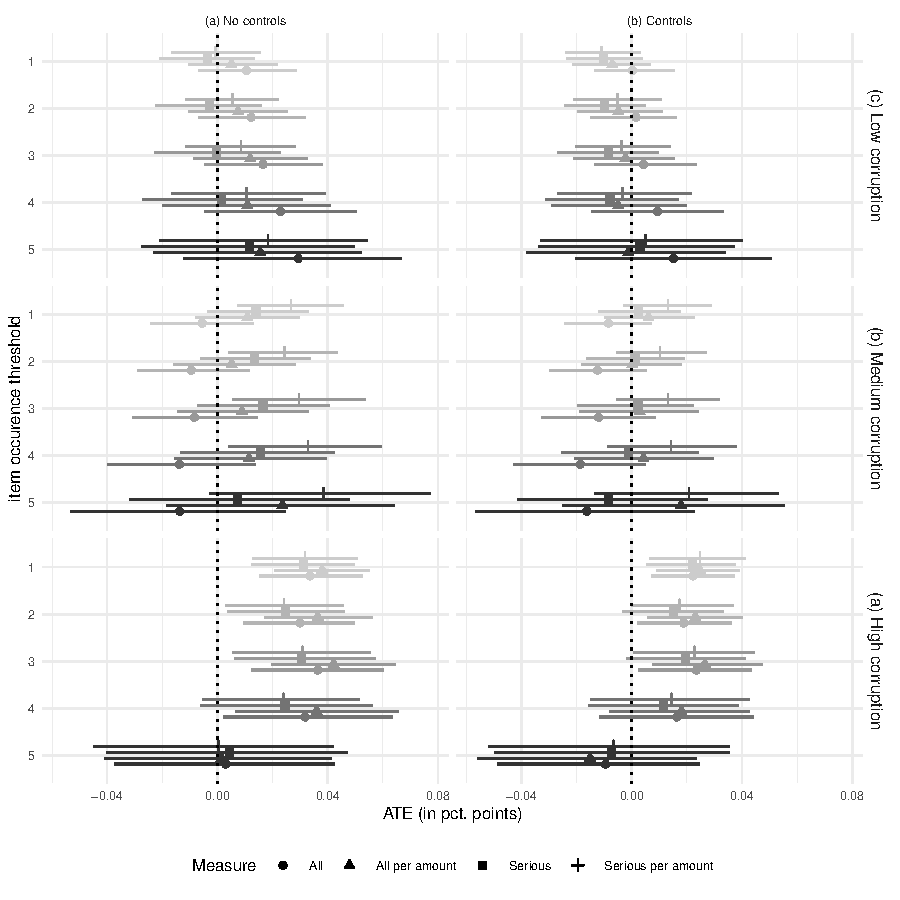
\includegraphics{chapters/chapter_2/figures/mgmtRobust.pdf}
    \caption{{\bf Robustness of findings on management to alternative specifications of the management index.} This figure reproduces the bottom panel of Figure \ref{fig:mainPl}, but varies the the minimum number of occurrences necessary to include an item in the management index from 1 (threshold used in Figure \ref{fig:mainPl}) to 5. Findings are robust up to a threshold of 3 occurrences.}
    \label{fig:managementRobustness}
\end{figure}

\subsection{Subset of never audited municipalities}
\label{app:neverAuditedRobustness}

Some municipalities in our sample have been audited prior to 2006, the starting year of the period we consider in the study. This robustness check reestimates our models on the subset of municipalities that have been audited between 2006 and 2015, but have never been audited before, and finds similar results.

\begin{figure}[H]
    \centering
    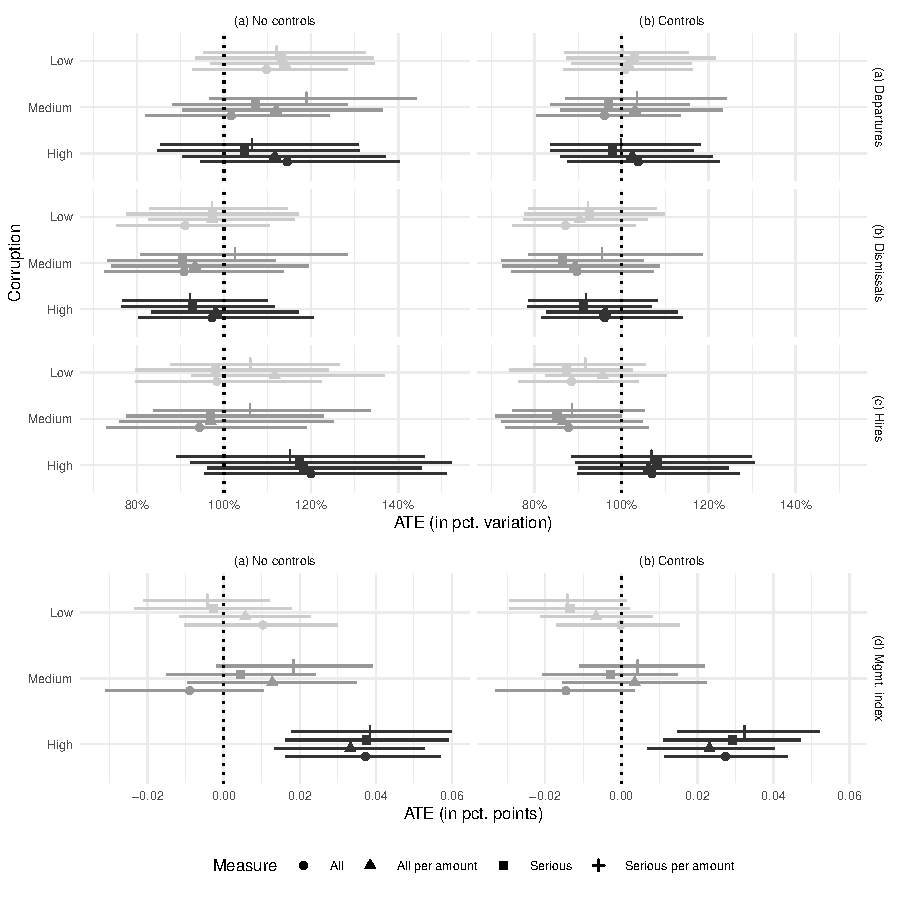
\includegraphics{chapters/chapter_2/figures/plSubsetMun}
    \caption{{\bf Subset of never audited municipalities only.} This figure reproduces Figure \ref{fig:mainPl} in the main text but considers only those municipalities that have never been audited before 2006.}
    \label{fig:plSubsetMun}
\end{figure}


\subsection{Individual-level analysis}
\label{app:multinomial}

The aggregated models we estimated in the previous section do not take full advantage of our micro-data, and separate departures from dismissals. We estimate instead a multi-outcome, discrete-time survival model in which bureaucrats may leave the bureaucracy either voluntarily or by being dismissed, and find again that audits have little effect on career interruptions. 

Career interruptions may have two causes: dismissals and voluntary departures. Yet, those two events have a very different nature, since dismissals are imposed upon employees by management, while departures are voluntary, or mandated by some life event (e.g. injury or retirement). As such, they might respond differently to treatment. We investigate the possibility by considering a discrete-time multi-outcome proportional hazard model. It turns out that this model reduces to a multinomial logistic regression with year fixed effects. We take equation \ref{eq:base} to the individual level, defining the outcome $y_{ijst} = 0$ if bureaucrat $i$ is employed by the end of year $t$, $y_{ijst} = 1$ if $i$ departed during year $t$, and $y_{ijst} = 2$ if $i$ was dismissed during year $t$. 

These models yield two sets of parameters that quantify the impact of each variable on, in turn, the (log-)odds of departure ($y_{ijst} = 1$) and dismissal ($y_{ijst} = 2$) relative to no career interruption ($y_{ijst} = 0$). Since generalized linear models are highly sensitive to model misspecification, all our specifications include controls. We add to the municipal-level controls used in our main specifications a number of individual-level controls that are either time-invariant or follow a deterministic evolution; namely, gender, education, contract type, years of work experience, and age.\footnote{That is, log number of employees in 2006 and their median wage, municipality-level illiteracy rate, urbanization rate and gini measured in the 2001 census, and the number of audited items. Our education variable contains the levels ``none,'' ``primary school,'' ``middle school,'' ``high school,'' and ``higher education.'' The contract type variable is a binary variable that separates tenured from untenured contracts.} Furthermore, since we compare bureaucrats that were affected by the audit to bureaucrats, in the same year, in municipalities that have not been audited yet, we only consider those bureaucrats that entered (and possibly left) the bureaucracy before the audit. In other words, we discard those employees that entered the bureaucracy after the audit, since this event may have been affected by treatment. Additionally, we compare within cohort by adding a cohort fixed effect. 

Table \ref{tbl:modsMultinom} reports the results, and confirms that audit have no discernible effect on career interruptions. None of the coefficients of interest are consistently different from zero across corruption metrics. Furthermore, the ones that are point at a modest \emph{chilling} effect, showing that audits lead to decreases the probability of departure and dismissal in moderate-corruption municipality (models 1 and 3), or in high-corruption municipalities (model 4). 


\begin{table}[H]
    \centering
    \footnotesize
	{
\def\sym#1{\ifmmode^{#1}\else\(^{#1}\)\fi}
\begin{tabular}{l*{4}{c}}
\toprule
                    &\multicolumn{1}{c}{(1)}&\multicolumn{1}{c}{(2)}&\multicolumn{1}{c}{(3)}&\multicolumn{1}{c}{(4)}\\
                    &\multicolumn{1}{c}{All faults}&\multicolumn{1}{c}{Serious faults}&\multicolumn{1}{c}{All faults}&\multicolumn{1}{c}{Serious faults}\\
                    &\multicolumn{1}{c}{}&\multicolumn{1}{c}{}&\multicolumn{1}{c}{normalized}&\multicolumn{1}{c}{normalized}\\
\midrule
$\beta_1$ - departure&                     &                     &                     &                     \\
\addlinespace
treat ($\beta_{11}$)            &       0.136         &      0.0777         &      0.0835         &       0.204         \\
                    &      (0.96)         &      (0.57)         &      (0.68)         &      (1.53)         \\

moderate corruption        &       0.462\sym{*}  &       0.348         &       0.153         &       0.284\sym{*}  \\
                    &      (2.16)         &      (1.84)         &      (0.67)         &      (2.05)         \\
high corruption        &       0.241         &       0.223         &       0.127         &       0.539\sym{*}  \\
                    &      (1.02)         &      (0.97)         &      (0.68)         &      (2.39)         \\
treat $\times$ moderate corruption ($\beta_{21}$)&      -0.412\sym{*}  &      -0.180         &      -0.368         &      -0.255         \\
                    &     (-2.23)         &     (-0.95)         &     (-1.81)         &     (-1.48)         \\
treat $\times$ high corruption ($\beta_{31}$)&     -0.0119         &      -0.156         &      -0.206         &      -0.867\sym{***}\\
                    &     (-0.05)         &     (-0.69)         &     (-1.25)         &     (-3.75)         \\
\midrule
$\beta_2$ - dismissal&                     &                     &                     &                     \\
\addlinespace
treat ($\beta_{12}$)             &     -0.0109         &       0.224         &      -0.165         &      -0.125         \\
                    &     (-0.08)         &      (1.50)         &     (-1.08)         &     (-0.81)         \\
moderate corruption        &       0.221         &       0.351\sym{*}  &     -0.0332         &       0.266         \\
                    &      (1.42)         &      (2.32)         &     (-0.17)         &      (1.35)         \\
high corruption        &       0.104         &       0.339         &      -0.414\sym{*}  &      0.0762         \\
                    &      (0.42)         &      (1.39)         &     (-2.03)         &      (0.34)         \\
treat $\times$ moderate corruption ($\beta_{22}$)&      -0.138         &      -0.492\sym{*}  &      0.0290         &      0.0779         \\
                    &     (-0.68)         &     (-2.25)         &      (0.14)         &      (0.37)         \\
treat $\times$ high corruption ($\beta_{32}$)&      -0.187         &      -0.650\sym{*}  &       0.273         &      -0.127         \\
                    &     (-0.81)         &     (-2.53)         &      (1.34)         &     (-0.52)         \\
\midrule
$\beta_{11} + \beta_{21}$& $-0.276^{**} $ & $-0.102 $ & $-0.284^{**} $ & $-0.052 $ \\
$\beta_{11} + \beta_{31}$& $0.124 $ & $-0.078 $ & $-0.122 $ & $-0.663^{***} $ \\
$\beta_{12} + \beta_{22}$& $-0.149^{**} $ & $-0.268 $ & $-0.136^{**} $ & $-0.047 $ \\
$\beta_{12} + \beta_{32}$& $-0.198 $ & $-0.426 $ & $0.108 $ & $-0.252^{***} $ \\
Observations        &      448493         &      448493         &      448493         &      448493         \\
\textit{AIC}        &    357677.3         &    357656.9         &    357975.0         &    357270.2         \\
\bottomrule
\multicolumn{5}{l}{\footnotesize \textit{t} statistics in parentheses}\\
\multicolumn{5}{l}{\footnotesize \sym{*} \(p<0.05\), \sym{**} \(p<0.01\), \sym{***} \(p<0.001\)}\\
\end{tabular}
}

	\caption{{\bf Treatment effect with multiple outcomes.} Coefficients are odds ratios from multinomial logistic regression models with 95 percent confidence intervals clustered at the municipality-level. The 4 rows that add parameters report the sum of the parameters, with stars corresponding to the p-value of the associated $\chi^2$ test. All models include year, state, and cohort fixed effects and the controls discussed in this section. Audits have no effect on career interruption that is consistent across all corruption metrics. If anything, results points at a moderate chilling effect: audits reduce the probability of departure and dismissal in moderate-corruption municipality (models 1 and 3), or in high-corruption municipalities (model 4).}
	\label{tbl:modsMultinom}
\end{table}


\subsection{Political models with other corruption metrics}
\label{app:political}

In this section, we reproduce the model reported in Figure \ref{fig:AMEpolitical1} of the main text using different metrics for corruption. We also report, for all such metrics, a model that tracks the effect of audits on the cohort hired by an incumbent mayor in the first year of her first term, after she has lost the election and is replaced by her challenger. For those models, the x-axis reports the electoral years of the challenger's term, while the colors refer to the year of the incumbent's term during which the audit ocurred. All specifications point towards the same conclusion that despite there being evidence of seasonality in staff rotation, with spikes in hiring and career interruptions around election years, audits do not significantly affect this pattern. 

\subsubsection*{First term}

 \begin{figure}[H]
     \centering
     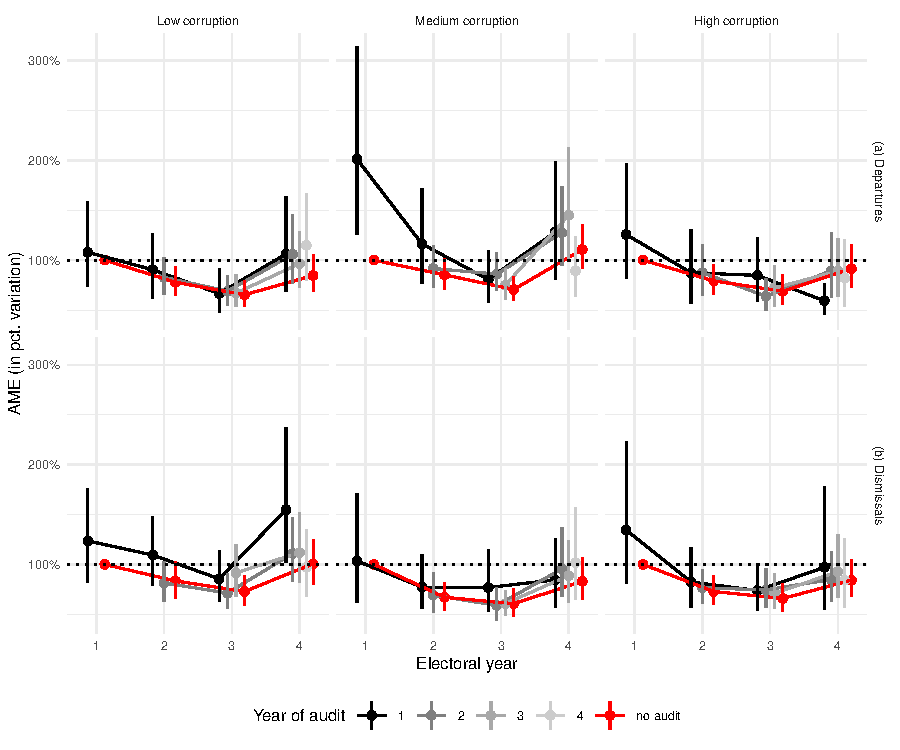
\includegraphics{chapters/chapter_2/figures/AMEpoliticalSerious_term1Client.pdf}
     \caption{{\bf Treatment effect as a function of the political cycle during the incumbent's term, corruption = \# serious faults.} This figure reproduces Figure \ref{fig:AMEpolitical1} in the main text but uses \# serious faults as a measure of corruption.}
     \label{fig:AMEpolitical1_serious}
 \end{figure}

 \begin{figure}[H]
    \centering
    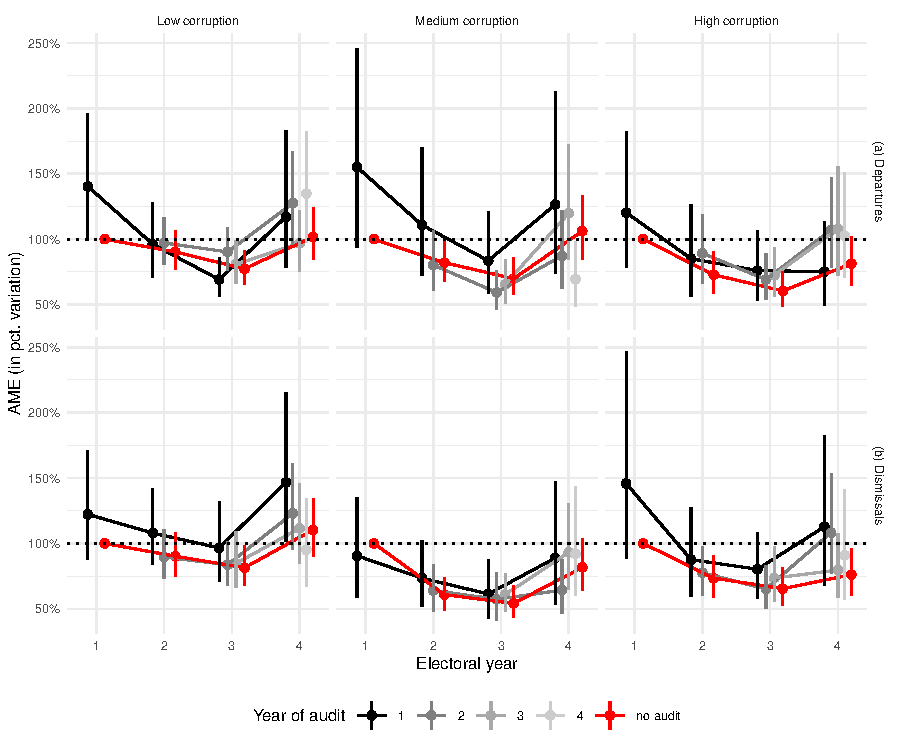
\includegraphics{chapters/chapter_2/figures/AMEpoliticalAllPerAMount_term1Client.pdf}
    \caption{{\bf Treatment effect as a function of the political cycle during the incumbent's term, corruption = total \# faults per amount audited.} This figure reproduces Figure \ref{fig:AMEpolitical1} in the main text but uses total \# faults per amount audited as a measure of corruption.}
    \label{fig:AMEpolitical1_allPerAmount}
\end{figure}

\begin{figure}[H]
    \centering
    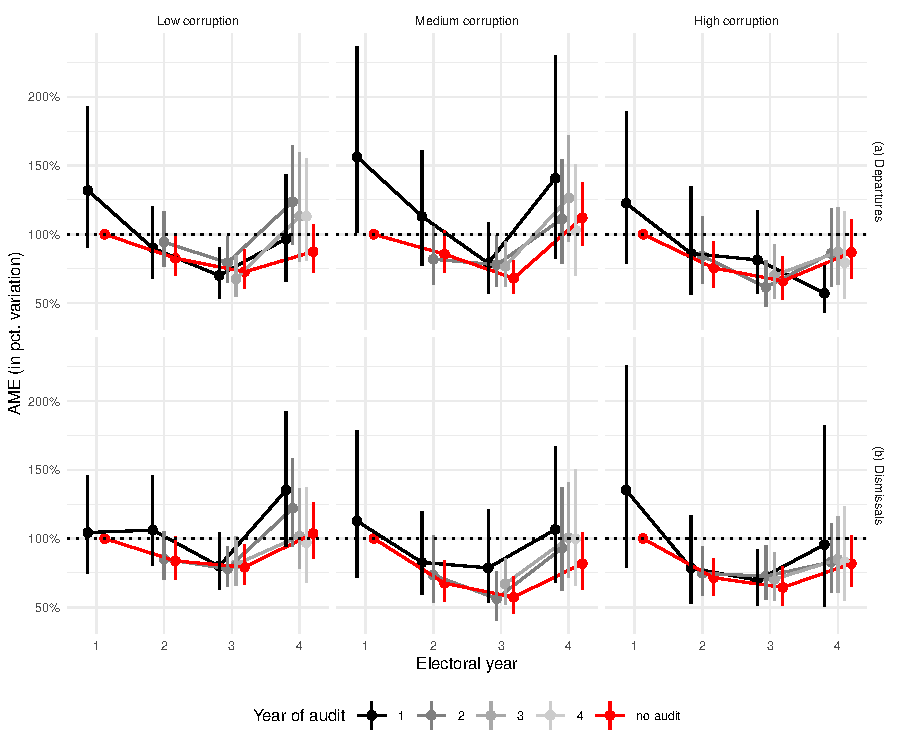
\includegraphics{chapters/chapter_2/figures/AMEpoliticalSeriousPerAmount_term1Client.pdf}
    \caption{{\bf Treatment effect as a function of the political cycle during the incumbent's term, corruption = total \# faults per amount audited.} This figure reproduces Figure \ref{fig:AMEpolitical1} in the main text but uses total \# faults per amount audited as a measure of corruption.}
    \label{fig:AMEpolitical1_seriousPerAmount}
\end{figure}

\subsubsection*{Second term}

\begin{figure}[H]
    \centering
    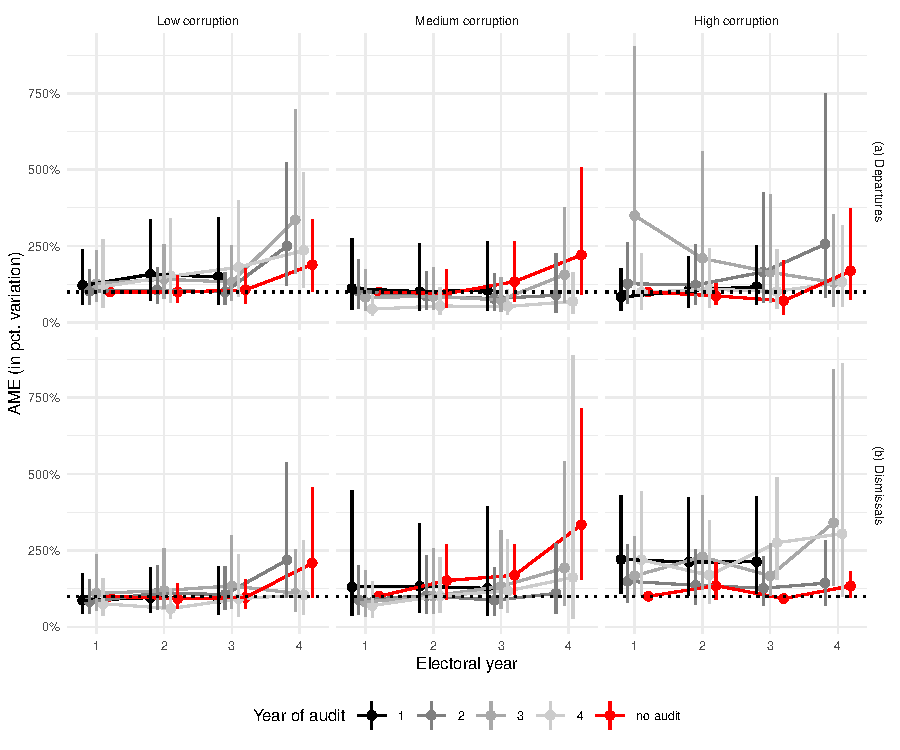
\includegraphics{chapters/chapter_2/figures/AMEpolitical_term2Client.pdf}
    \caption{{\bf Treatment effect as a function of the political cycle during the challenger's term} The y-axis represents the average marginal effect of audits the row outcome. The x-axis represents years in the political cycle, with year 1 being the first year of mandate. Colors indicate the year of the political cycle during which the audit occurred. Bars are 95 percent confidence intervals clustered at the municipality level. All models use the controls discussed in section \ref{sub:empiricalStrategy}. Again, we find no evidence that anti-corruption audits induce any changes in bureaucratic personnel.}
    \label{fig:AMEpolitical2}
\end{figure}

\begin{figure}[H]
    \centering
    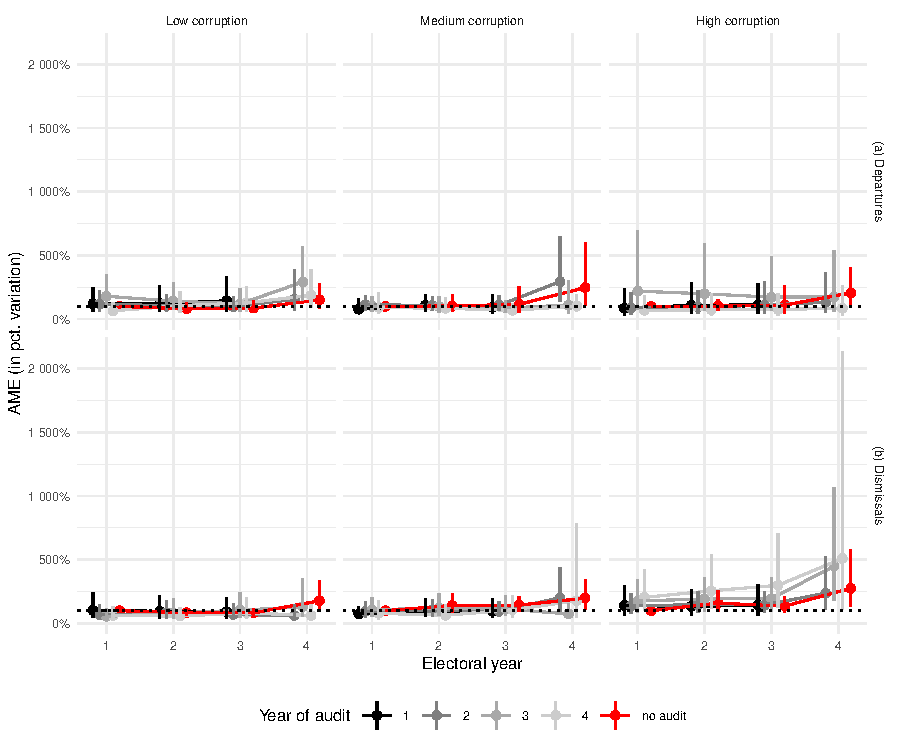
\includegraphics{chapters/chapter_2/figures/AMEpoliticalSerious_term2Client.pdf}
    \caption{{\bf Treatment effect as a function of the political cycle during the challenger's term, corruption = \# serious faults.} This figure reproduces Figure \ref{fig:AMEpolitical2} above but uses \# serious faults as a measure of corruption.}
    \label{fig:AMEpolitical2_serious}
\end{figure}

\begin{figure}[H]
   \centering
   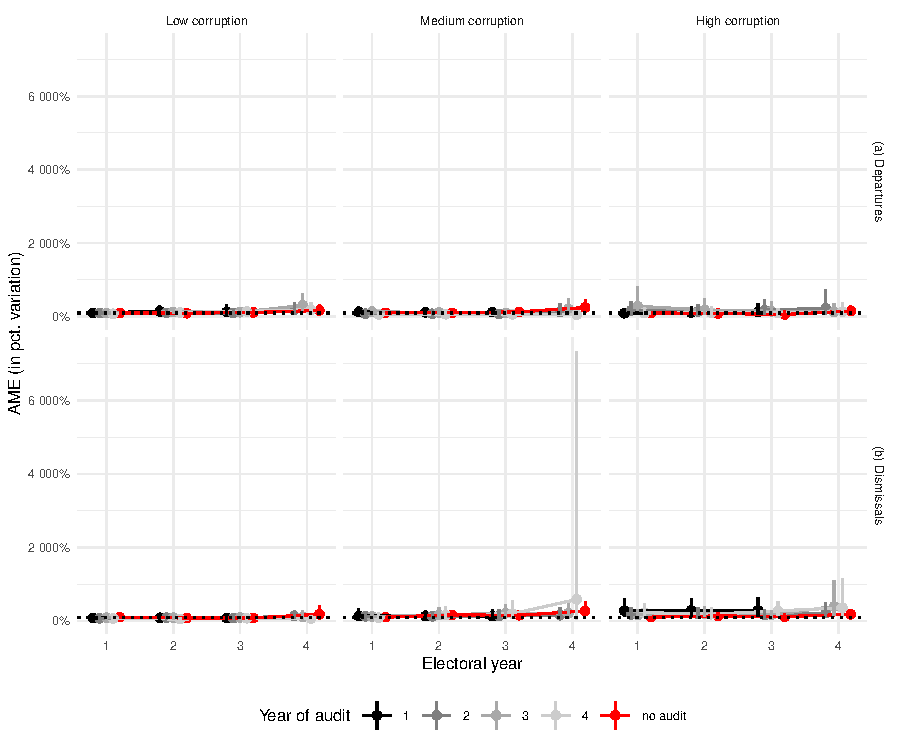
\includegraphics{chapters/chapter_2/figures/AMEpoliticalAllPerAMount_term2Client.pdf}
   \caption{{\bf Treatment effect as a function of the political cycle during the challenger's term, corruption = total \# faults per amount audited.} This figure reproduces Figure \ref{fig:AMEpolitical2} above but uses total \# faults per amount audited as a measure of corruption.}
   \label{fig:AMEpolitical2_allPerAmount}
\end{figure}

\begin{figure}[H]
   \centering
   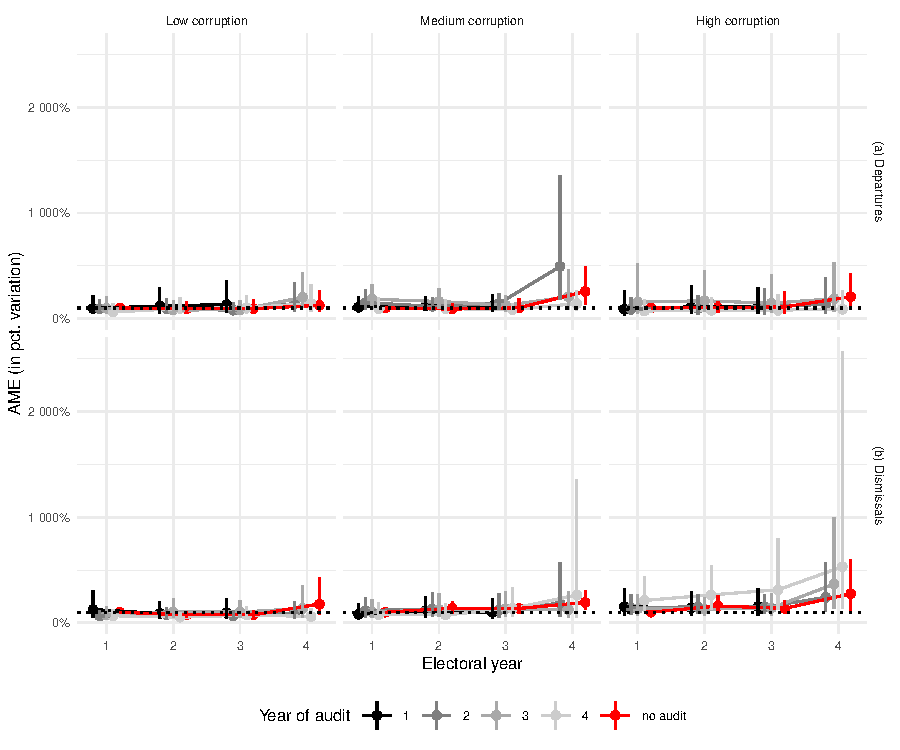
\includegraphics{chapters/chapter_2/figures/AMEpoliticalSeriousPerAmount_term2Client.pdf}
   \caption{{\bf Treatment effect as a function of the political cycle during the challenger's term, corruption = total \# faults per amount audited.} This figure reproduces Figure \ref{fig:AMEpolitical2} above but uses total \# faults per amount audited as a measure of corruption.}
   \label{fig:AMEpolitical2_seriousPerAmount}
\end{figure}

\section{Estimation and validation of the DDC model}
\label{app:structural}

In this section, we first report the auxiliary models used in estimating the DDC model reported in Section \ref{sec:structural}, and show results from a validation exercise (Figure \ref{fig:validationStructuralSize}). 

Recall that the vector of individual-level parameters is $\theta_i = (\delta_i, p_i, w_i, \wb_i, k_i)$. Estimating parameter $p$ is straightforward: since $p$ is the probability of an audit in a given year, we simply use the probability of an audit in each state as per the lottery procedure. Other parameters are more challenging, largely because these parameters are time-invariant, while our data structure is time-varying. As such, we turn parameters that are essentially time-varying into time-invariant parameters by predicting their value for individual $i$ with characteristics $x_i$ over its lifecycle; that is, from the first year this person is observed in the dataset until mandatory retirement age. Vector $x_i$ includes time-invariant characteristics such as gender, education, the municipal-level controls used in the reduced-form models (section \ref{sec:causal}), state-level fixed effects, as well as deterministic time-varying variables such as age and work experience. 

We estimate the discount factor $\delta$ by predicting the probability of individual $i$ retiring from the labor market using a logistic regression. We estimate public and private-sector wages $w_i$ and $\wb_i$ using the Blinder-Oaxaca procedure \citep{blinder1973wage}; i.e. we regress the (log) wages of public sector employees over predictors $x_i$, and estimate a second model for private sector employees.\footnote{Predictors include education, age, gender, work experience.} Parameter $w_i$ is therefore the average salary of employee $i$ if she stayed in the public sector from the first year we observe her until retirement, while $\wb_i$ is the average salary of employee $i$ should she depart to the private sector on the first year we observe her until retirement. Finally, we estimate the dismissal penalty $k$ by comparing, for an individual with characteristics $x_i$, the private sector wage $\wb_1$ that follows a voluntary departure to the private sector wage $\wb_2$ that follows a dismissal and obtain $k_i$ by averaging those differences of the individual's lifecycle from the first year we observe her until retirement. That is, we have $k_i = \frac{1}{t_i} \sum_{t=1}^{t_i} \widehat{\wb_2(i,t)} - \widehat{\wb_1(i,t)}$, with $t_i$ the number of years until $i$ retires.

\begin{figure}[H]
    \centering
    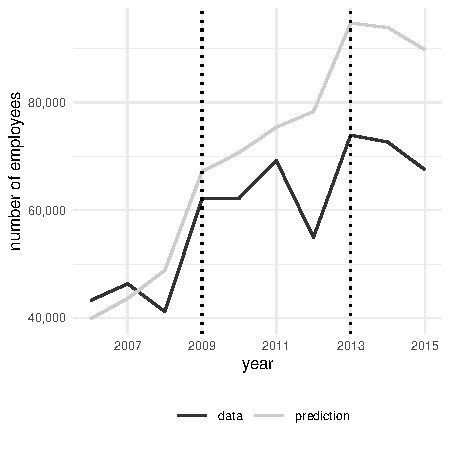
\includegraphics{chapters/chapter_2/figures/validationStructuralSize.pdf}
    \caption{{\bf Validation.} Comparing variation in the size of the bureaucracy as observed in the data and as predicted by our estimates, we find that predictions match reality remarkably well, except in years 2008 and 2012, which are pre-electoral years during which large waves of dismissals and departures occur.}
    \label{fig:validationStructuralSize}
\end{figure}